\section{Lineare Funktionen – Geraden verstehen}
\label{sec:lineare_funktionen_ueberarbeitet}

\begin{aufgabenumgebung}{Funktionsmaschinen-Logik}{}
Stell dir die folgenden Funktionsmaschinen vor. Gib jeweils die Funktionsgleichung $f(x) = \dots$ an, die beschreibt, was die Maschine mit der Eingabe $x$ macht.
\begin{enumerate}
    \item Maschine M1: Verdoppelt die Eingabe $x$ und addiert anschließend 5.
    \item Maschine M2: Subtrahiert von der Eingabe $x$ die Zahl 7 und multipliziert das Ergebnis mit 3.
    \item Maschine M3: Multipliziert die Eingabe $x$ mit sich selbst (quadriert sie) und zieht dann 4 ab.
    \item Maschine M4: Addiert zur Eingabe $x$ die Zahl 2, dividiert das Ergebnis durch 4 und addiert dann $x$.
\end{enumerate}
\end{aufgabenumgebung}


\begin{loesungsumgebung}[loes:funktionsmaschinen]{Funktionsmaschinen-Logik}
Um die Funktionsgleichungen $f(x)$ für die gegebenen Maschinen zu finden, übersetzen wir die beschriebenen Rechenschritte systematisch in mathematische Ausdrücke. Die Eingabe wird als $x$ bezeichnet.

\begin{enumerate}
    \item \textbf{Maschine M1: Verdoppelt die Eingabe $x$ und addiert anschließend 5.}
    \begin{itemize}
        \item \textbf{Schritt 1:} Die Eingabe $x$ wird verdoppelt: $2 \cdot x = 2x$.
        \item \textbf{Schritt 2:} Zu diesem Ergebnis wird 5 addiert: $2x + 5$.
    \end{itemize}
    Somit lautet die Funktionsgleichung für Maschine M1:
    $f(x) = 2x + 5$.

    \item \textbf{Maschine M2: Subtrahiert von der Eingabe $x$ die Zahl 7 und multipliziert das Ergebnis mit 3.}
    \begin{itemize}
        \item \textbf{Schritt 1:} Von der Eingabe $x$ wird 7 subtrahiert: $x - 7$.
        \item \textbf{Schritt 2:} Das Ergebnis $(x-7)$ wird mit 3 multipliziert: $3 \cdot (x - 7)$.
    \end{itemize}
    Die Funktionsgleichung für Maschine M2 ist:
    $f(x) = 3(x - 7)$.
    Man kann dies auch ausmultiplizieren zu $f(x) = 3x - 21$.

    \item \textbf{Maschine M3: Multipliziert die Eingabe $x$ mit sich selbst (quadriert sie) und zieht dann 4 ab.}
    \begin{itemize}
        \item \textbf{Schritt 1:} Die Eingabe $x$ wird mit sich selbst multipliziert (quadriert): $x \cdot x = x^2$.
        \item \textbf{Schritt 2:} Von diesem Ergebnis wird 4 abgezogen: $x^2 - 4$.
    \end{itemize}
    Die Funktionsgleichung für Maschine M3 lautet:
    $f(x) = x^2 - 4$.

    \item \textbf{Maschine M4: Addiert zur Eingabe $x$ die Zahl 2, dividiert das Ergebnis durch 4 und addiert dann $x$.}
    \begin{itemize}
        \item \textbf{Schritt 1:} Zur Eingabe $x$ wird 2 addiert: $x + 2$.
        \item \textbf{Schritt 2:} Das Ergebnis $(x+2)$ wird durch 4 dividiert: $\frac{x+2}{4}$.
        \item \textbf{Schritt 3:} Zu diesem Ergebnis wird $x$ addiert: $\frac{x+2}{4} + x$.
    \end{itemize}
    Die Funktionsgleichung für Maschine M4 ist:
    $f(x) = \frac{x+2}{4} + x$.
    Diese Gleichung kann noch vereinfacht werden:
    $f(x) = \frac{x+2}{4} + \frac{4x}{4} = \frac{x+2+4x}{4} = \frac{5x+2}{4}$.
    Alternativ kann man schreiben: $f(x) = \frac{5}{4}x + \frac{2}{4} = \frac{5}{4}x + \frac{1}{2}$.
\end{enumerate}

\begin{tippumgebung}{Text in Mathematik übersetzen}
Das Aufstellen von Funktionsgleichungen aus Textbeschreibungen ist eine wichtige Fähigkeit. Achte genau auf Schlüsselwörter:
\begin{itemize}
    \item 'addieren', 'summe', 'vermehrt um' bedeuten $+$.
    \item 'subtrahieren', 'differenz', 'vermindert um', 'zieht ab' bedeuten $-$.
    \item 'multiplizieren', 'produkt', 'mal', 'vervielfacht' bedeuten $\cdot$.
    \item 'dividieren', 'quotient', 'geteilt durch' bedeuten $: $ oder $\frac{\dots}{\dots}$.
    \item 'das Ergebnis' oder 'davon' deutet oft auf die Notwendigkeit von Klammern hin, um die Reihenfolge der Operationen korrekt wiederzugeben (Punkt- vor Strichrechnung beachten!).
\end{itemize}
Übe, die beschriebenen Schritte nacheinander in mathematische Terme umzuwandeln.
\end{tippumgebung}

\end{loesungsumgebung}

\begin{aufgabenumgebung}{Werte aus der Maschine}{}
Gegeben sind die folgenden Funktionsmaschinen durch ihre Funktionsgleichungen. Welche Ausgabe $f(x)$ (oder $y$) erzeugt die Maschine, wenn die angegebene Zahl $x$ eingegeben wird?
\begin{enumerate}
    \item $f(x) = 4x - 7$
    \begin{itemize}
        \item Was kommt raus bei $x=3$?
        \item Was kommt raus bei $x=0$?
        \item Was kommt raus bei $x=-2$?
    \end{itemize}
    \item $g(x) = -2(x+3)$
    \begin{itemize}
        \item Was kommt raus bei $x=1$?
        \item Was kommt raus bei $x=-3$?
        \item Was kommt raus bei $x=-5$?
    \end{itemize}
\end{enumerate}
\end{aufgabenumgebung}


\begin{loesungsumgebung}[loes:werte-aus-maschine]{Werte aus der Maschine}
Um die Ausgabe $f(x)$ (oder $y$) der Funktionsmaschinen zu bestimmen, setzen wir die gegebenen $x$-Werte in die jeweilige Funktionsgleichung ein und berechnen das Ergebnis.

\begin{enumerate}
    \item \textbf{Funktionsmaschine $f(x) = 4x - 7$}
    \begin{itemize}
        \item \textbf{Was kommt raus bei $x=3$?} \\
        Wir setzen $x=3$ in die Funktionsgleichung ein:
        $f(3) = 4 \cdot (3) - 7$
        $f(3) = 12 - 7$
        $f(3) = 5$ \\
        \textbf{Antwort:} Bei $x=3$ kommt $5$ raus.

        \item \textbf{Was kommt raus bei $x=0$?} \\
        Wir setzen $x=0$ in die Funktionsgleichung ein:
        $f(0) = 4 \cdot (0) - 7$
        $f(0) = 0 - 7$
        $f(0) = -7$ \\
        \textbf{Antwort:} Bei $x=0$ kommt $-7$ raus.

        \item \textbf{Was kommt raus bei $x=-2$?} \\
        Wir setzen $x=-2$ in die Funktionsgleichung ein:
        $f(-2) = 4 \cdot (-2) - 7$
        $f(-2) = -8 - 7$
        $f(-2) = -15$ \\
        \textbf{Antwort:} Bei $x=-2$ kommt $-15$ raus.
    \end{itemize}

    \item \textbf{Funktionsmaschine $g(x) = -2(x+3)$}
    \begin{itemize}
        \item \textbf{Was kommt raus bei $x=1$?} \\
        Wir setzen $x=1$ in die Funktionsgleichung ein:
        $g(1) = -2 \cdot (1+3)$
        $g(1) = -2 \cdot (4)$
        $g(1) = -8$ \\
        \textbf{Antwort:} Bei $x=1$ kommt $-8$ raus.

        \item \textbf{Was kommt raus bei $x=-3$?} \\
        Wir setzen $x=-3$ in die Funktionsgleichung ein:
        $g(-3) = -2 \cdot (-3+3)$
        $g(-3) = -2 \cdot (0)$
        $g(-3) = 0$ \\
        \textbf{Antwort:} Bei $x=-3$ kommt $0$ raus.

        \item \textbf{Was kommt raus bei $x=-5$?} \\
        Wir setzen $x=-5$ in die Funktionsgleichung ein:
        $g(-5) = -2 \cdot (-5+3)$
        $g(-5) = -2 \cdot (-2)$
        $g(-5) = 4$ \\
        \textbf{Antwort:} Bei $x=-5$ kommt $4$ raus.
    \end{itemize}
\end{enumerate}

\begin{tippumgebung}{Sorgfältiges Rechnen}
Achte beim Einsetzen von Werten in Funktionsgleichungen besonders auf:
\begin{itemize}
    \item \textbf{Klammern:} Setze negative Zahlen oder Terme, die aus mehreren Teilen bestehen (wie $(x+3)$ in $g(x)$), beim Einsetzen und Multiplizieren ggf. in Klammern, um Vorzeichenfehler zu vermeiden.
    \item \textbf{Rechenreihenfolge:} Beachte die Regel 'Punktrechnung vor Strichrechnung' und die korrekte Auswertung von Klammern. Bei $g(x) = -2(x+3)$ wird zuerst die Klammer $(x+3)$ berechnet und dann das Ergebnis mit $-2$ multipliziert.
    \item \textbf{Vorzeichen:} Sei besonders wachsam bei Rechnungen mit negativen Zahlen. $- \cdot - = +$, $+ \cdot - = -$.
\end{itemize}
Ein schrittweises Vorgehen hilft, Fehler zu minimieren.
\end{tippumgebung}

\end{loesungsumgebung}

\begin{aufgabenumgebung}{Steigung zwischen zwei Punkten}
Berechne die Steigung der Geraden, die durch die folgenden Punktepaare verläuft. Versuche auch, dir vorzustellen oder zu skizzieren, wie die Gerade ungefähr aussieht (steigend/fallend, steil/flach).
\begin{enumerate}
    \item $A(-1|1)$ und $B(2|7)$
    \item $C(0|4)$ und $D(3|1)$
    \item $E(-2|-3)$ und $F(4|-3)$ (Was ist hier besonders?)
    \item $G(2|1)$ und $H(2|5)$ (Was ist hier besonders? Ist das noch eine Funktion $y=f(x)$? Begründe!)
\end{enumerate}
\end{aufgabenumgebung}


\begin{loesungsumgebung}[loes:steigung-zwei-punkte]{Steigung zwischen zwei Punkten}
Die Steigung $m$ einer Geraden, die durch zwei Punkte $P_1(x_1|y_1)$ und $P_2(x_2|y_2)$ verläuft, wird mit der folgenden Formel berechnet:
$$ m = \frac{\Delta y}{\Delta x} = \frac{y_2 - y_1}{x_2 - x_1} $$
Diese Formel gibt das Verhältnis der Veränderung in der $y$-Richtung zur Veränderung in der $x$-Richtung an.

\begin{enumerate}
    \item \textbf{Punkte $A(-1|1)$ und $B(2|7)$} \\
    Hier ist $x_1 = -1$, $y_1 = 1$ und $x_2 = 2$, $y_2 = 7$.
    $$ m = \frac{7 - 1}{2 - (-1)} = \frac{6}{2 + 1} = \frac{6}{3} = 2 $$
    \textbf{Interpretation:} Die Steigung ist $m=2$. Da $m > 0$, ist die Gerade steigend. Für jede Einheit, die man auf der $x$-Achse nach rechts geht, geht es 2 Einheiten auf der $y$-Achse nach oben. Die Gerade ist relativ steil.

    \item \textbf{Punkte $C(0|4)$ und $D(3|1)$} \\
    Hier ist $x_1 = 0$, $y_1 = 4$ und $x_2 = 3$, $y_2 = 1$.
    $$ m = \frac{1 - 4}{3 - 0} = \frac{-3}{3} = -1 $$
    \textbf{Interpretation:} Die Steigung ist $m=-1$. Da $m < 0$, ist die Gerade fallend. Für jede Einheit, die man auf der $x$-Achse nach rechts geht, geht es 1 Einheit auf der $y$-Achse nach unten. Die Gerade fällt in einem 45°-Winkel.

    \item \textbf{Punkte $E(-2|-3)$ und $F(4|-3)$} \\
    Hier ist $x_1 = -2$, $y_1 = -3$ und $x_2 = 4$, $y_2 = -3$.
    $$ m = \frac{-3 - (-3)}{4 - (-2)} = \frac{-3 + 3}{4 + 2} = \frac{0}{6} = 0 $$
    \textbf{Was ist hier besonders?} Die Steigung ist $m=0$.
    \textbf{Interpretation:} Eine Steigung von Null bedeutet, dass die Gerade horizontal verläuft. Sie ist parallel zur $x$-Achse. Alle Punkte auf dieser Geraden haben denselben $y$-Wert (hier $y=-3$).

    \item \textbf{Punkte $G(2|1)$ und $H(2|5)$} \\
    Hier ist $x_1 = 2$, $y_1 = 1$ und $x_2 = 2$, $y_2 = 5$.
    $$ m = \frac{5 - 1}{2 - 2} = \frac{4}{0} $$
    \textbf{Was ist hier besonders?} Der Nenner ist Null, was bedeutet, dass die Steigung nicht definiert ist (Division durch Null).
    \textbf{Interpretation:} Eine undefinierte Steigung bedeutet, dass die Gerade vertikal verläuft. Sie ist parallel zur $y$-Achse. Alle Punkte auf dieser Geraden haben denselben $x$-Wert (hier $x=2$).
    \textbf{Ist das noch eine Funktion $y=f(x)$? Begründe!}
    Nein, eine vertikale Gerade (außer sie wäre die $y$-Achse selbst, und auch dann nur eingeschränkt) ist im Allgemeinen \textbf{keine Funktion} der Form $y=f(x)$.
    \textbf{Begründung:} Bei einer Funktion $y=f(x)$ muss jedem $x$-Wert genau ein $y$-Wert zugeordnet sein. Bei dieser Geraden wird dem $x$-Wert $x=2$ jedoch mehr als ein $y$-Wert zugeordnet (z.B. $y=1$ und $y=5$). Dies verletzt die Definition einer Funktion.
\end{enumerate}

\begin{merksatzumgebung}{Interpretation der Steigung $m$}
Die Steigung $m$ einer Geraden gibt an, wie stark und in welche Richtung sich die Gerade verändert:
\begin{itemize}
    \item $m > 0$: Die Gerade steigt von links nach rechts an. Je größer $m$, desto steiler.
    \item $m < 0$: Die Gerade fällt von links nach rechts ab. Je kleiner (d.h. je größer der Betrag von $m$), desto steiler fällt sie.
    \item $m = 0$: Die Gerade ist horizontal (parallel zur $x$-Achse). Die $y$-Werte ändern sich nicht.
    \item $m$ ist undefiniert (Division durch Null im Steigungsbruch): Die Gerade ist vertikal (parallel zur $y$-Achse). Die $x$-Werte ändern sich nicht. Dies ist keine Funktion $y=f(x)$.
\end{itemize}
\end{merksatzumgebung}

\begin{center}
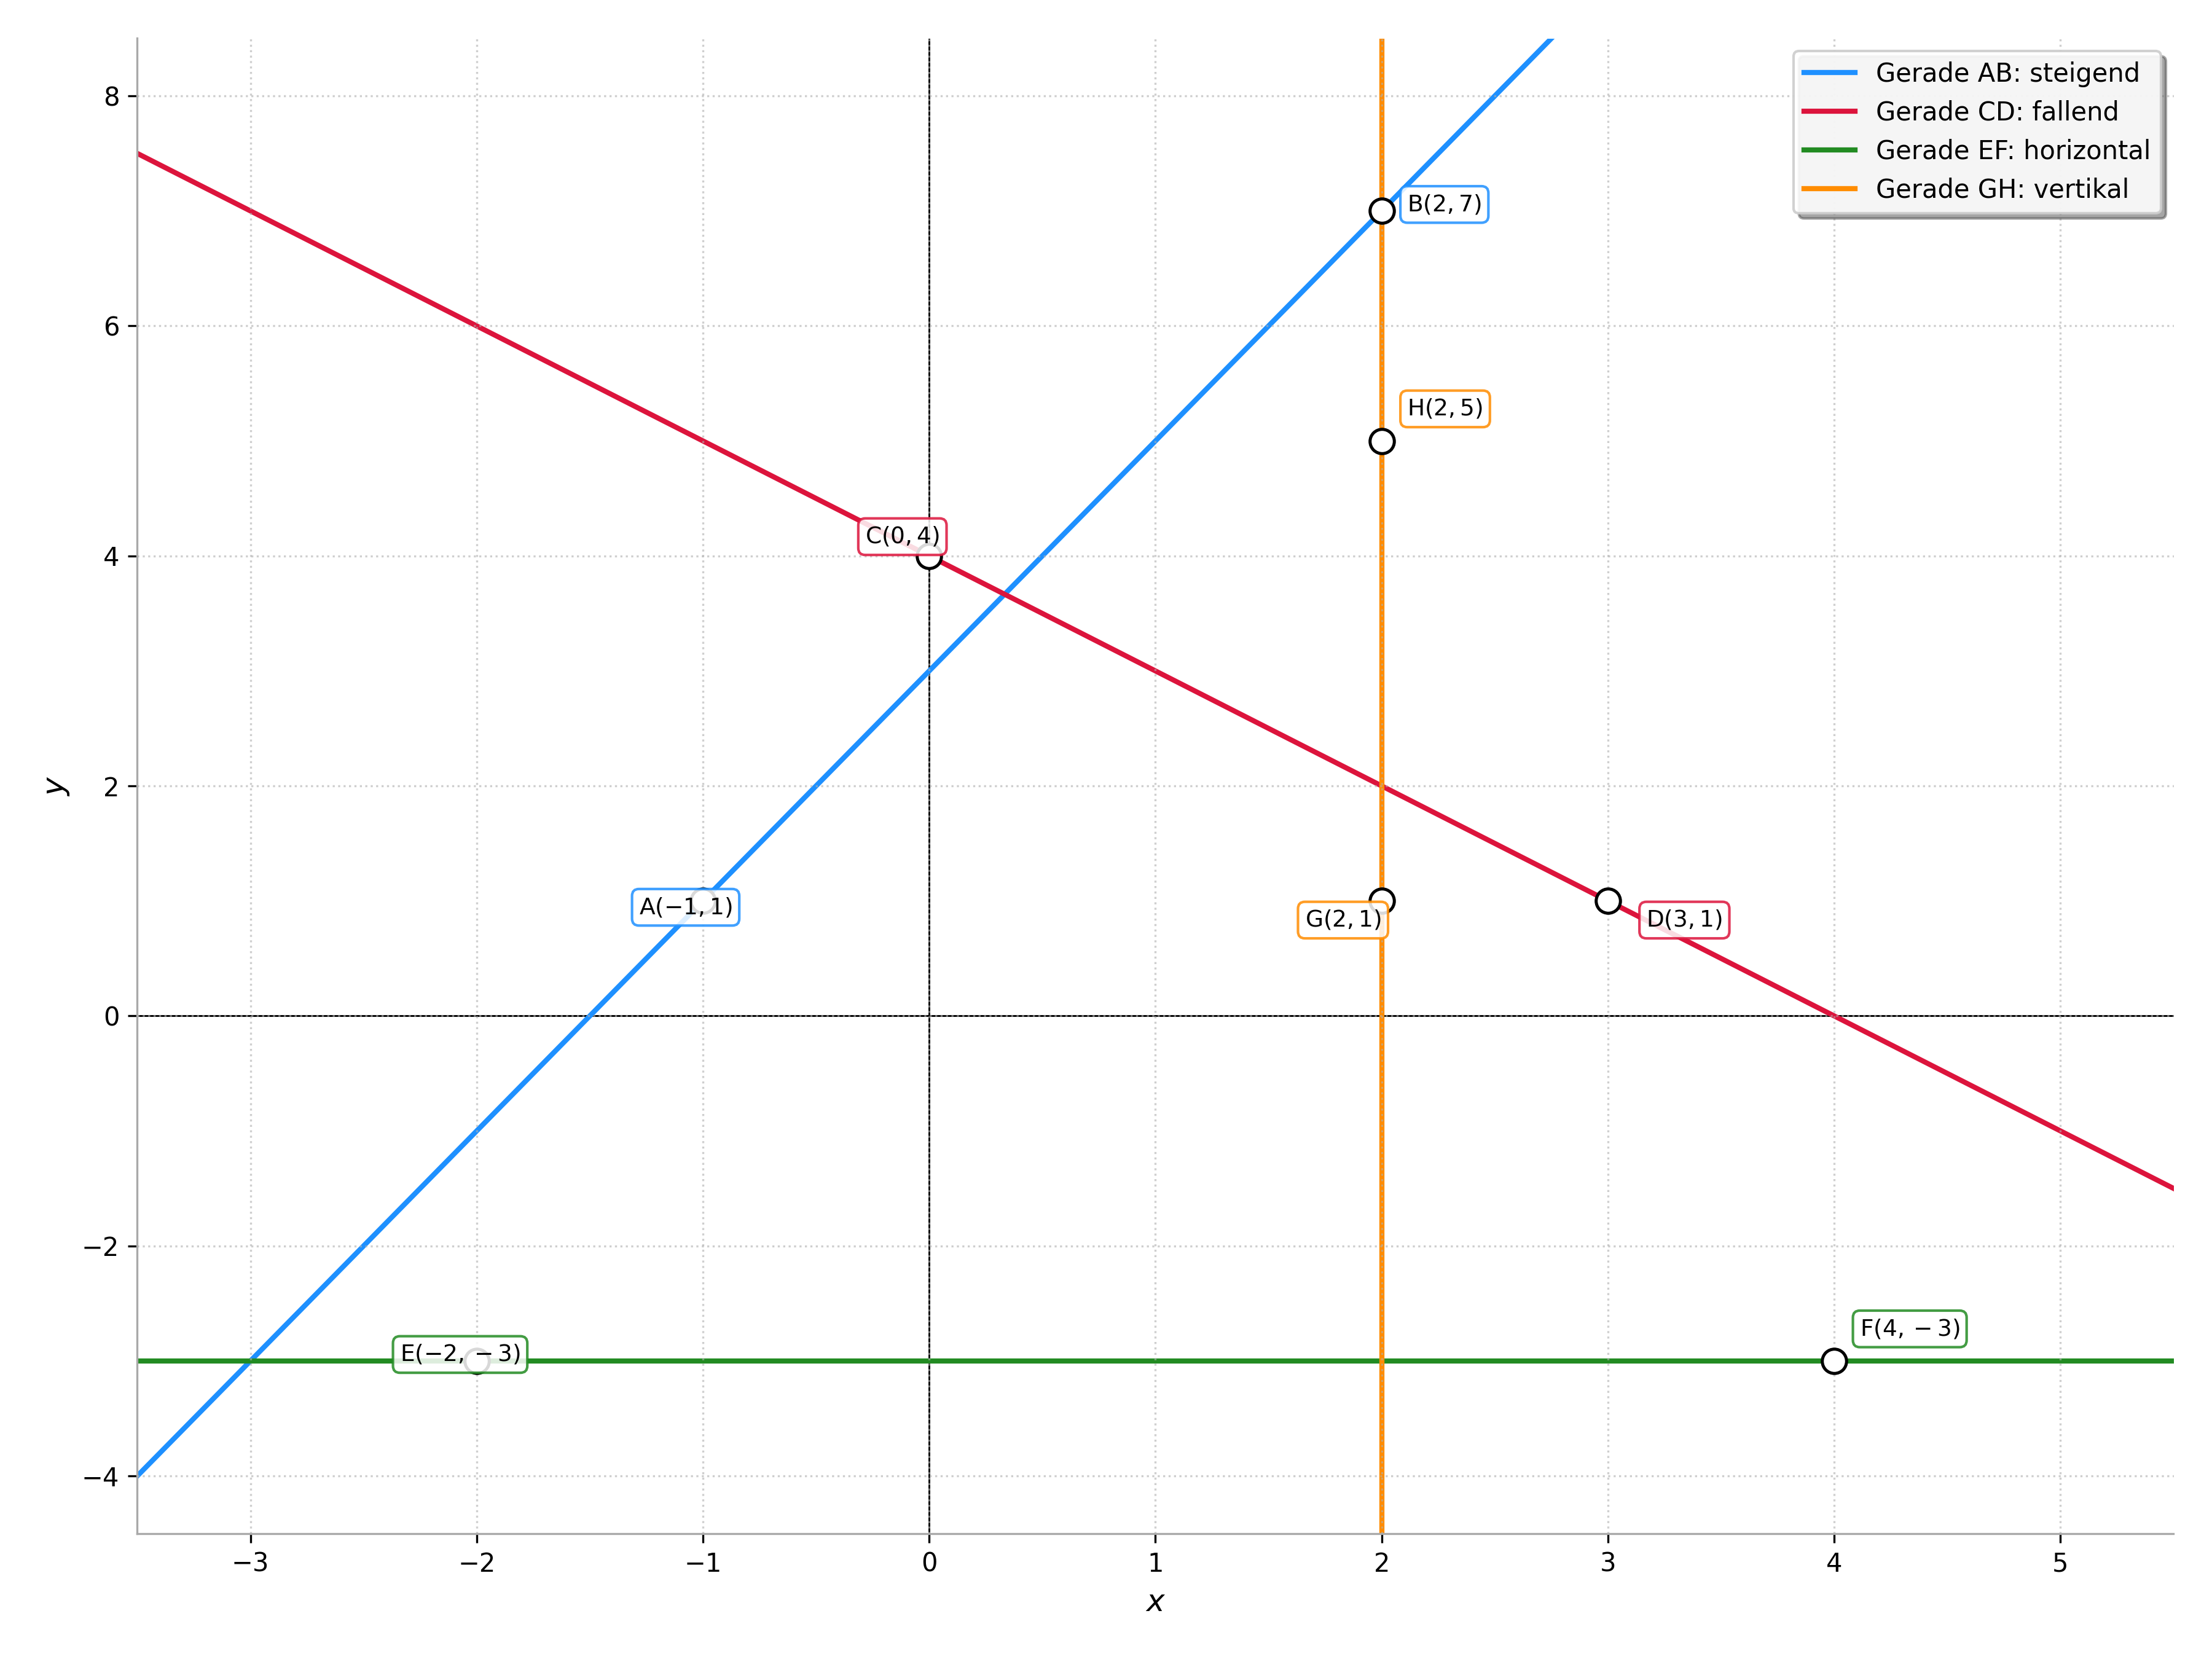
\includegraphics[width=0.9\textwidth]{grafiken/steigung_punkte_skizze.png}
% --- Beschreibung der Grafik, die hier erscheinen soll ---
% Die Grafik sollte ein Koordinatensystem zeigen, in dem die vier Geraden skizziert sind:
% 1. Gerade AB: Durch A(-1|1) und B(2|7), klar steigend.
% 2. Gerade CD: Durch C(0|4) und D(3|1), fallend.
% 3. Gerade EF: Durch E(-2|-3) und F(4|-3), horizontal.
% 4. Gerade GH: Durch G(2|1) und H(2|5), vertikal.
% Jeder Punkt sollte beschriftet sein, und die Geraden könnten farblich unterschieden oder ebenfalls beschriftet werden.
% Alternativ können auch vier separate kleine Koordinatensysteme für jede Gerade gezeichnet werden.
% Wichtig ist die visuelle Darstellung der unterschiedlichen Steigungsarten.
\captionof{figure}{Skizzen der Geraden durch die gegebenen Punktepaare zur Veranschaulichung der Steigungen.}
\label{fig:steigung_skizzen}
\end{center}

\end{loesungsumgebung}



\begin{aufgabenumgebung}{Lineare Funktionen umfassend bestimmen und analysieren}

\textbf{Teil 1: Gerade mit positiver Steigung} \\
Gegeben sind die Punkte $C(-2|0)$ und $D(2|8)$, durch die eine lineare Funktion $f(x) = ax+b$ verläuft.

\begin{enumerate}[label=(\alph*)]
    \item \textbf{Steigung berechnen:} Berechne die Steigung $a$ der Geraden durch die Punkte C und D.
    \item \textbf{Y-Achsenabschnitt berechnen:} Bestimme den y-Achsenabschnitt $b$ der Geraden.
    \item \textbf{Funktionsgleichung aufstellen:} Gib die vollständige Funktionsgleichung $f(x)$ an.
    \item \textbf{Nullstelle bestimmen:} Berechne die Nullstelle $x_N$ der Funktion $f(x)$. Welcher der gegebenen Punkte entspricht der Nullstelle?
    \item \textbf{Funktionswerte berechnen:}
        \begin{itemize}
            \item Welchen Wert hat $f(0)$? Was sagt dieser Wert über den Graphen aus?
            \item Berechne $f(1)$.
        \end{itemize}
    \item \textbf{Argument für einen Funktionswert finden:} Für welchen Wert von $x$ gilt $f(x) = 6$?
    \item \textbf{Punktprobe:} Liegt der Punkt $P(3|10)$ auf der Geraden? Begründe deine Antwort rechnerisch.
    \item \textbf{Skizze und Überprüfung:} Zeichne den Graphen der Funktion $f(x)$ in ein Koordinatensystem. Markiere die Punkte C und D sowie den y-Achsenabschnitt und die Nullstelle. Überprüfe anhand deiner Zeichnung, ob deine berechneten Werte für $a$ (Steigungsdreieck) und $b$ plausibel sind.
    \item \textbf{Vorzeichen der Funktionswerte:} Was kannst du über das Vorzeichen der Funktionswerte $f(x)$ sagen für $x$-Werte, die kleiner als die Nullstelle sind ($x < x_N$), und für $x$-Werte, die größer als die Nullstelle sind ($x > x_N$)? Begründe dies anhand der Steigung und der Nullstelle.
\end{enumerate}

\bigskip % Fügt einen größeren vertikalen Abstand ein

\textbf{Teil 2: Gerade mit negativer Steigung} \\
Gegeben sind die Punkte $E(-1|3)$ und $F(1|-1)$, durch die eine lineare Funktion $g(x) = ax+b$ verläuft.

\begin{enumerate}[label=(\alph*)]
    \item \textbf{Steigung berechnen:} Berechne die Steigung $a$ der Geraden durch die Punkte E und F.
    \item \textbf{Y-Achsenabschnitt berechnen:} Bestimme den y-Achsenabschnitt $b$ der Geraden.
    \item \textbf{Funktionsgleichung aufstellen:} Gib die vollständige Funktionsgleichung $g(x)$ an.
    \item \textbf{Nullstelle bestimmen:} Berechne die Nullstelle $x_N$ der Funktion $g(x)$.
    \item \textbf{Funktionswerte berechnen:}
        \begin{itemize}
            \item Welchen Wert hat $g(0)$? Was sagt dieser Wert über den Graphen aus?
            \item Berechne $g(3)$.
        \end{itemize}
    \item \textbf{Argument für einen Funktionswert finden:} Für welchen Wert von $x$ gilt $g(x) = 7$?
    \item \textbf{Punktprobe:} Liegt der Punkt $Q(0.5|0)$ auf der Geraden? Begründe deine Antwort rechnerisch. (Tipp: Vergleiche mit deiner Berechnung aus Teil d)).
    \item \textbf{Skizze und Überprüfung:} Zeichne den Graphen der Funktion $g(x)$ in ein Koordinatensystem. Markiere die Punkte E und F sowie den y-Achsenabschnitt und die Nullstelle. Überprüfe anhand deiner Zeichnung, ob deine berechneten Werte für $a$ (Ist die Gerade fallend? Wie ist das Steigungsdreieck?) und $b$ plausibel sind.
    \item \textbf{Vorzeichen der Funktionswerte:} Was kannst du über das Vorzeichen der Funktionswerte $g(x)$ sagen für $x$-Werte, die kleiner als die Nullstelle sind ($x < x_N$), und für $x$-Werte, die größer als die Nullstelle sind ($x > x_N$)? Begründe dies anhand der (negativen) Steigung und der Nullstelle.
\end{enumerate}
\end{aufgabenumgebung}


\begin{loesungsumgebung}[loes:lineare-funktionen-umfassend]{Lineare Funktionen umfassend bestimmen und analysieren}

\subsection*{Teil 1: Gerade mit positiver Steigung durch $C(-2|0)$ und $D(2|8)$}
Die allgemeine Form einer linearen Funktion ist $f(x) = ax+b$.

\begin{enumerate}[label=(\alph*)]
    \item \textbf{Steigung berechnen:}
    Die Punkte sind $C(-2|0)$ (also $x_1=-2, y_1=0$) und $D(2|8)$ (also $x_2=2, y_2=8$).
    Die Steigung $a$ berechnet sich als:
    $$ a = \frac{y_2 - y_1}{x_2 - x_1} = \frac{8 - 0}{2 - (-2)} = \frac{8}{2+2} = \frac{8}{4} = 2 $$
    Die Steigung ist $a=2$.

    \item \textbf{Y-Achsenabschnitt berechnen:}
    Wir setzen die Steigung $a=2$ und die Koordinaten eines Punktes (z.B. $D(2|8)$) in die Funktionsgleichung $f(x) = ax+b$ ein:
    $8 = 2 \cdot (2) + b$
    $8 = 4 + b$
    $b = 8 - 4 = 4$
    Der y-Achsenabschnitt ist $b=4$.

    \item \textbf{Funktionsgleichung aufstellen:}
    Mit $a=2$ und $b=4$ lautet die Funktionsgleichung:
    $f(x) = 2x + 4$.

    \item \textbf{Nullstelle bestimmen:}
    Die Nullstelle $x_N$ ist der $x$-Wert, für den $f(x_N)=0$ gilt:
    $2x_N + 4 = 0$
    $2x_N = -4$
    $x_N = -2$
    Die Nullstelle ist $x_N = -2$.
    Der gegebene Punkt $C(-2|0)$ entspricht der Nullstelle, da sein $y$-Wert 0 ist.

    \item \textbf{Funktionswerte berechnen:}
    \begin{itemize}
        \item Welchen Wert hat $f(0)$?
        $f(0) = 2 \cdot (0) + 4 = 0 + 4 = 4$.
        Was sagt dieser Wert über den Graphen aus? Der Wert $f(0)=4$ ist der y-Achsenabschnitt $b$. Er gibt an, dass der Graph die y-Achse im Punkt $(0|4)$ schneidet.
        \item Berechne $f(1)$.
        $f(1) = 2 \cdot (1) + 4 = 2 + 4 = 6$.
    \end{itemize}

    \item \textbf{Argument für einen Funktionswert finden:} Für welchen Wert von $x$ gilt $f(x) = 6$?
    $2x + 4 = 6$
    $2x = 6 - 4$
    $2x = 2$
    $x = 1$
    Für $x=1$ gilt $f(x)=6$.

    \item \textbf{Punktprobe:} Liegt der Punkt $P(3|10)$ auf der Geraden?
    Wir setzen $x=3$ in die Funktionsgleichung $f(x) = 2x+4$ ein:
    $f(3) = 2 \cdot (3) + 4 = 6 + 4 = 10$.
    Da der berechnete Funktionswert $10$ mit der y-Koordinate des Punktes $P$ übereinstimmt, liegt der Punkt $P(3|10)$ auf der Geraden.

    \item \textbf{Skizze und Überprüfung:}
    \begin{center}
    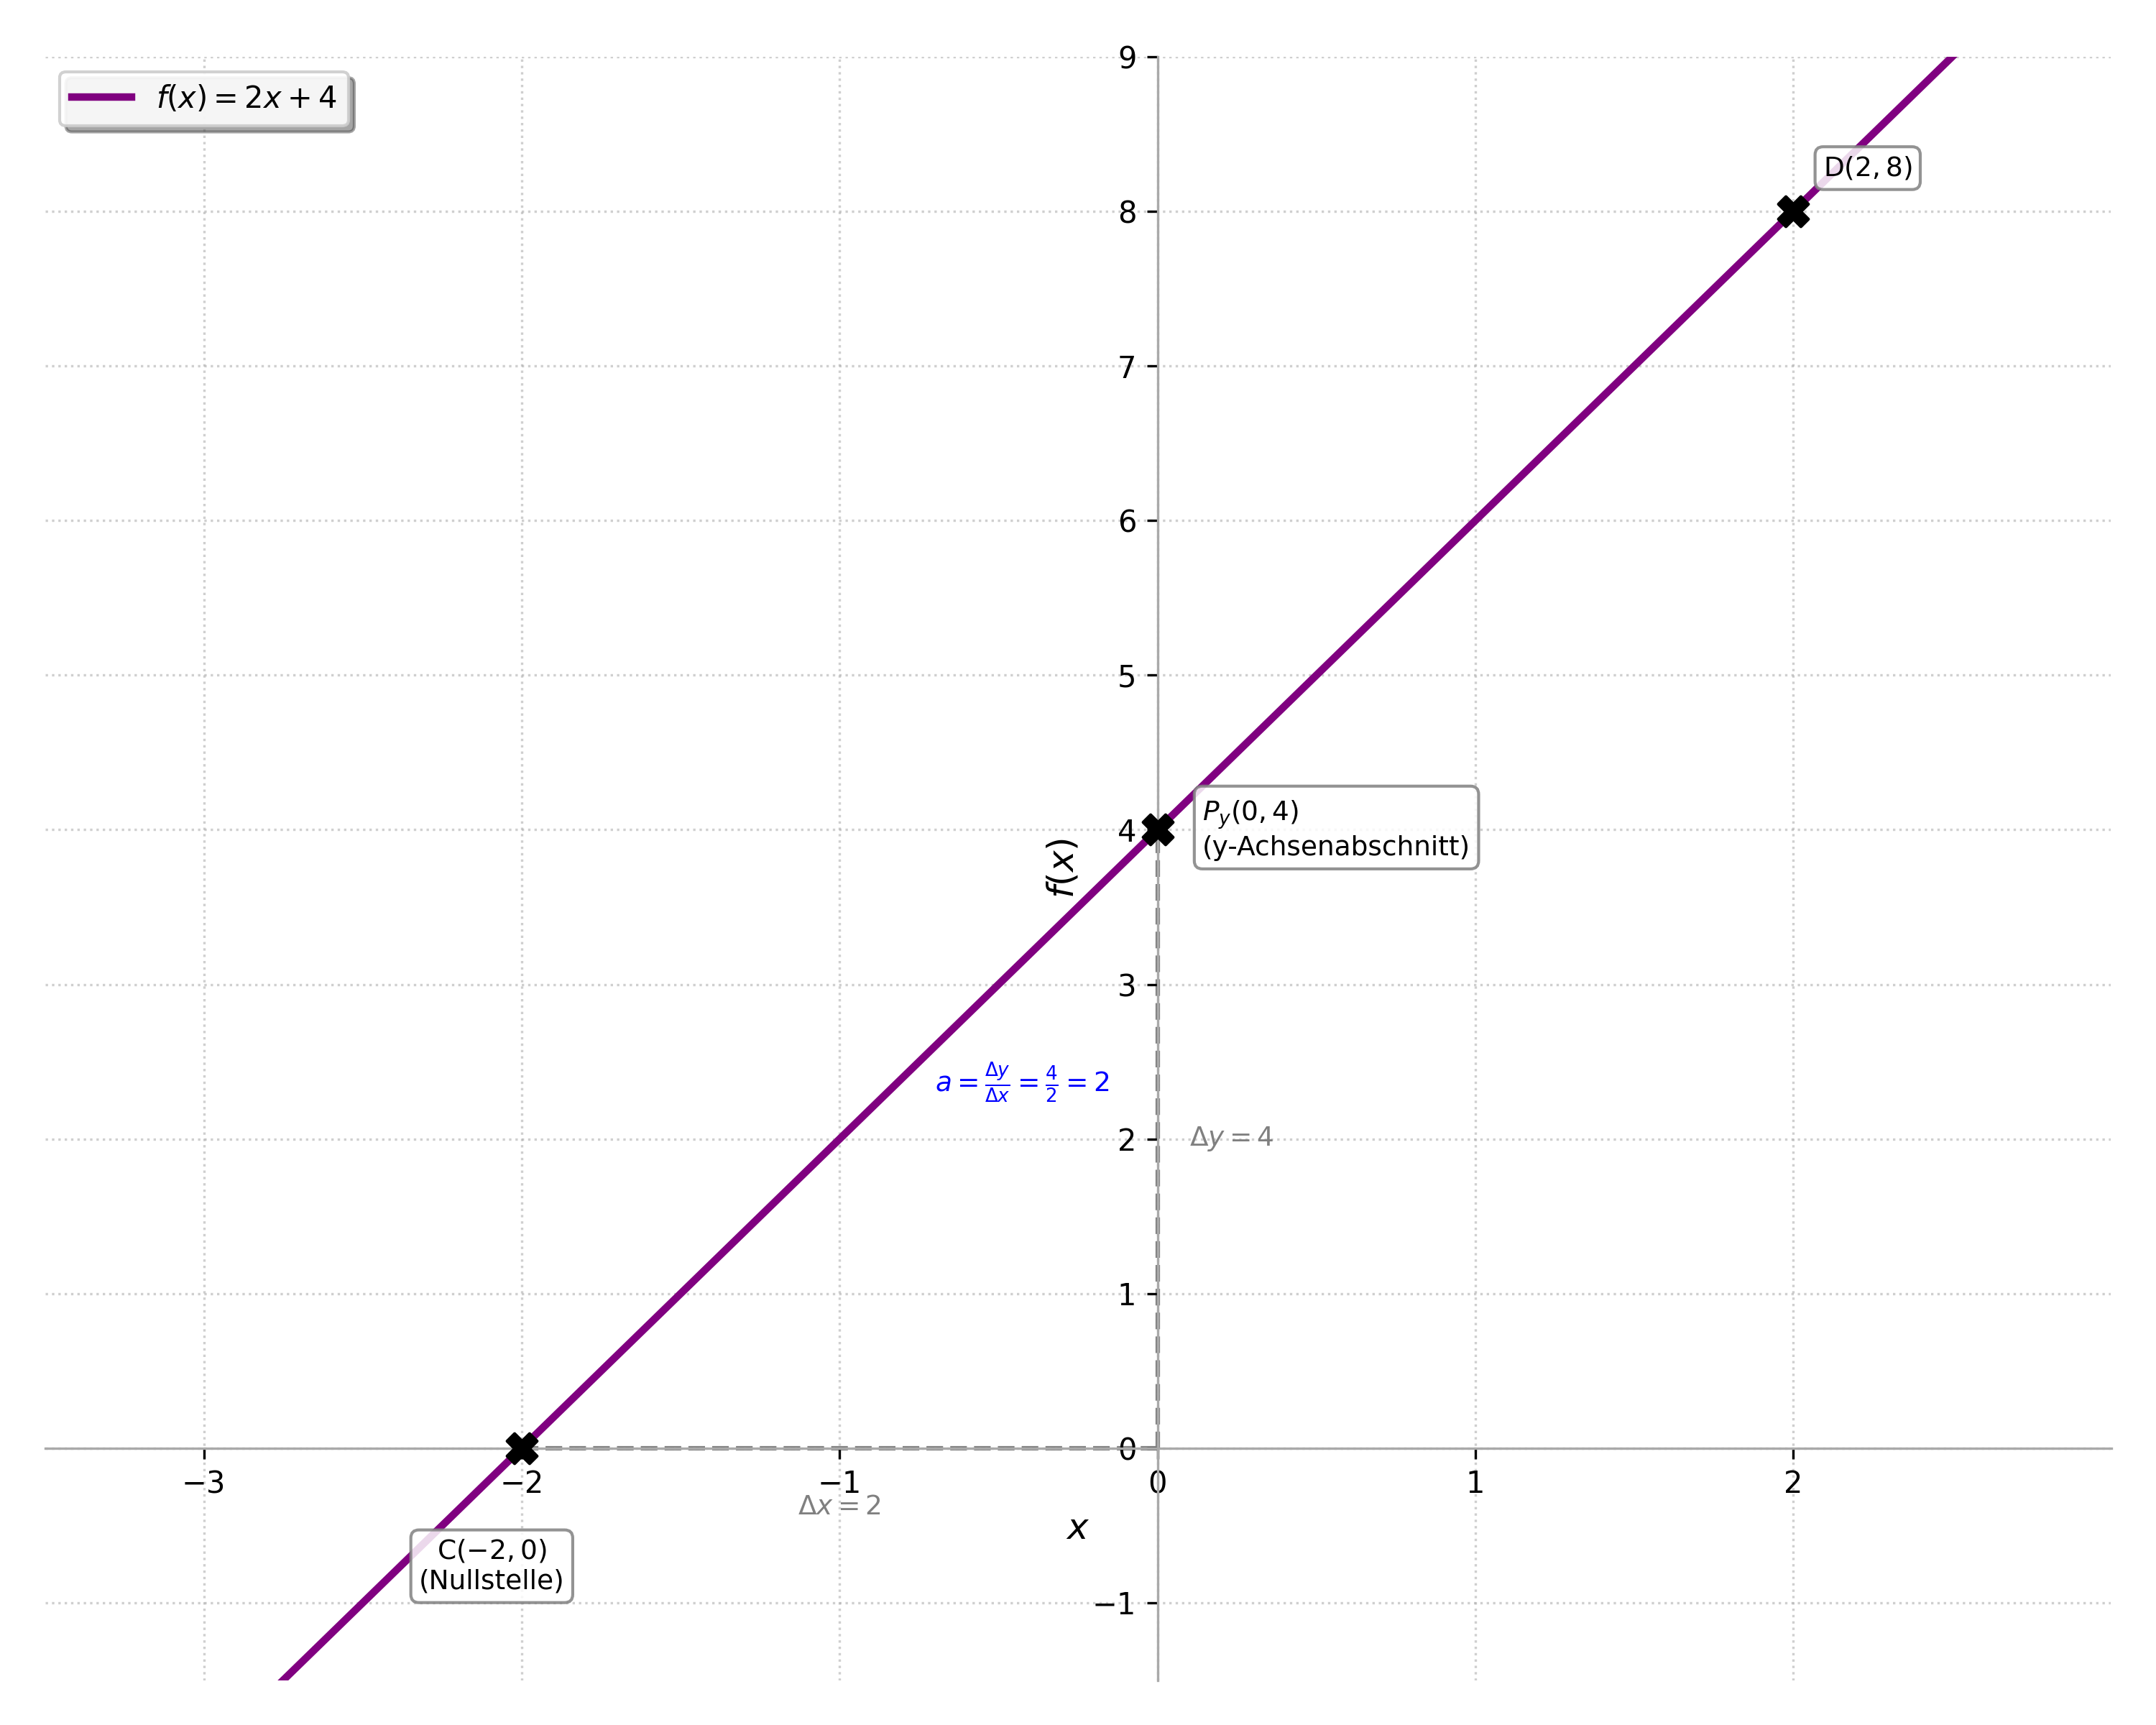
\includegraphics[width=0.8\textwidth]{grafiken/lin_fkt_teil1_skizze.png}
    % --- Beschreibung der Grafik für Teil 1 ---
    % Die Grafik sollte ein Koordinatensystem zeigen.
    % Eingezeichnet ist die Gerade f(x) = 2x + 4.
    % Die Punkte C(-2|0) und D(2|8) sind markiert.
    % Der y-Achsenabschnitt (0|4) ist markiert.
    % Die Nullstelle (-2|0) ist markiert (identisch mit Punkt C).
    % Ein Steigungsdreieck ist eingezeichnet, das die Steigung a=2 verdeutlicht (z.B. von C aus: 2 Einheiten nach rechts, 4 Einheiten nach oben bis (0|4), oder 1 Einheit nach rechts, 2 Einheiten nach oben).
    % Die Achsen sind beschriftet (x und y oder f(x)).
    \captionof{figure}{Skizze der Funktion $f(x)=2x+4$ mit Punkten C und D, y-Achsenabschnitt und Nullstelle.}
    \label{fig:lin_fkt_teil1}
    \end{center}
    \textbf{Überprüfung anhand der Skizze:} Man sollte erkennen, dass die Gerade durch die Punkte C und D verläuft. Der Schnittpunkt mit der y-Achse sollte bei $y=4$ liegen. Die Nullstelle (Schnittpunkt mit der x-Achse) sollte bei $x=-2$ liegen. Das Steigungsdreieck sollte eine Steigung von $a=2$ (z.B. 1 Einheit nach rechts, 2 Einheiten nach oben) visuell bestätigen. Die Gerade steigt an, was zu $a>0$ passt.

    \item \textbf{Vorzeichen der Funktionswerte:}
    Die Nullstelle ist $x_N = -2$ und die Steigung ist $a=2$ (positiv).
    \begin{itemize}
        \item Für $x < x_N$ (also $x < -2$): Die Funktionswerte $f(x)$ sind \textbf{negativ}. Da die Gerade steigt ($a>0$), kommt sie von 'unten links' und durchquert die x-Achse an der Nullstelle. Links von der Nullstelle liegen die Funktionswerte unterhalb der x-Achse. Z.B. $f(-3) = 2(-3)+4 = -2$.
        \item Für $x > x_N$ (also $x > -2$): Die Funktionswerte $f(x)$ sind \textbf{positiv}. Rechts von der Nullstelle liegen die Funktionswerte oberhalb der x-Achse. Z.B. $f(0) = 4$.
    \end{itemize}
\end{enumerate}

\bigskip % Vertikaler Abstand zwischen den Teilen

\subsection*{Teil 2: Gerade mit negativer Steigung durch $E(-1|3)$ und $F(1|-1)$}
Die allgemeine Form einer linearen Funktion ist $g(x) = ax+b$.

\begin{enumerate}[label=(\alph*)]
    \item \textbf{Steigung berechnen:}
    Die Punkte sind $E(-1|3)$ (also $x_1=-1, y_1=3$) und $F(1|-1)$ (also $x_2=1, y_2=-1$).
    Die Steigung $a$ berechnet sich als:
    $$ a = \frac{y_2 - y_1}{x_2 - x_1} = \frac{-1 - 3}{1 - (-1)} = \frac{-4}{1+1} = \frac{-4}{2} = -2 $$
    Die Steigung ist $a=-2$.

    \item \textbf{Y-Achsenabschnitt berechnen:}
    Wir setzen die Steigung $a=-2$ und die Koordinaten eines Punktes (z.B. $E(-1|3)$) in die Funktionsgleichung $g(x) = ax+b$ ein:
    $3 = -2 \cdot (-1) + b$
    $3 = 2 + b$
    $b = 3 - 2 = 1$
    Der y-Achsenabschnitt ist $b=1$.

    \item \textbf{Funktionsgleichung aufstellen:}
    Mit $a=-2$ und $b=1$ lautet die Funktionsgleichung:
    $g(x) = -2x + 1$.

    \item \textbf{Nullstelle bestimmen:}
    Die Nullstelle $x_N$ ist der $x$-Wert, für den $g(x_N)=0$ gilt:
    $-2x_N + 1 = 0$
    $-2x_N = -1$
    $x_N = \frac{-1}{-2} = \frac{1}{2}$ (oder $0.5$)
    Die Nullstelle ist $x_N = \frac{1}{2}$.

    \item \textbf{Funktionswerte berechnen:}
    \begin{itemize}
        \item Welchen Wert hat $g(0)$?
        $g(0) = -2 \cdot (0) + 1 = 0 + 1 = 1$.
        Was sagt dieser Wert über den Graphen aus? Der Wert $g(0)=1$ ist der y-Achsenabschnitt $b$. Er gibt an, dass der Graph die y-Achse im Punkt $(0|1)$ schneidet.
        \item Berechne $g(3)$.
        $g(3) = -2 \cdot (3) + 1 = -6 + 1 = -5$.
    \end{itemize}

    \item \textbf{Argument für einen Funktionswert finden:} Für welchen Wert von $x$ gilt $g(x) = 7$?
    $-2x + 1 = 7$
    $-2x = 7 - 1$
    $-2x = 6$
    $x = \frac{6}{-2} = -3$
    Für $x=-3$ gilt $g(x)=7$.

    \item \textbf{Punktprobe:} Liegt der Punkt $Q(0.5|0)$ auf der Geraden?
    Wir setzen $x=0.5$ in die Funktionsgleichung $g(x) = -2x+1$ ein:
    $g(0.5) = -2 \cdot (0.5) + 1 = -1 + 1 = 0$.
    Da der berechnete Funktionswert $0$ mit der y-Koordinate des Punktes $Q$ übereinstimmt, liegt der Punkt $Q(0.5|0)$ auf der Geraden.
    \textbf{Tipp-Vergleich:} Dies stimmt mit der Berechnung aus Teil d) überein, da $x_N=0.5$ die Nullstelle ist und $Q(0.5|0)$ somit der Nullstellenpunkt.

    \item \textbf{Skizze und Überprüfung:}
    \begin{center}
    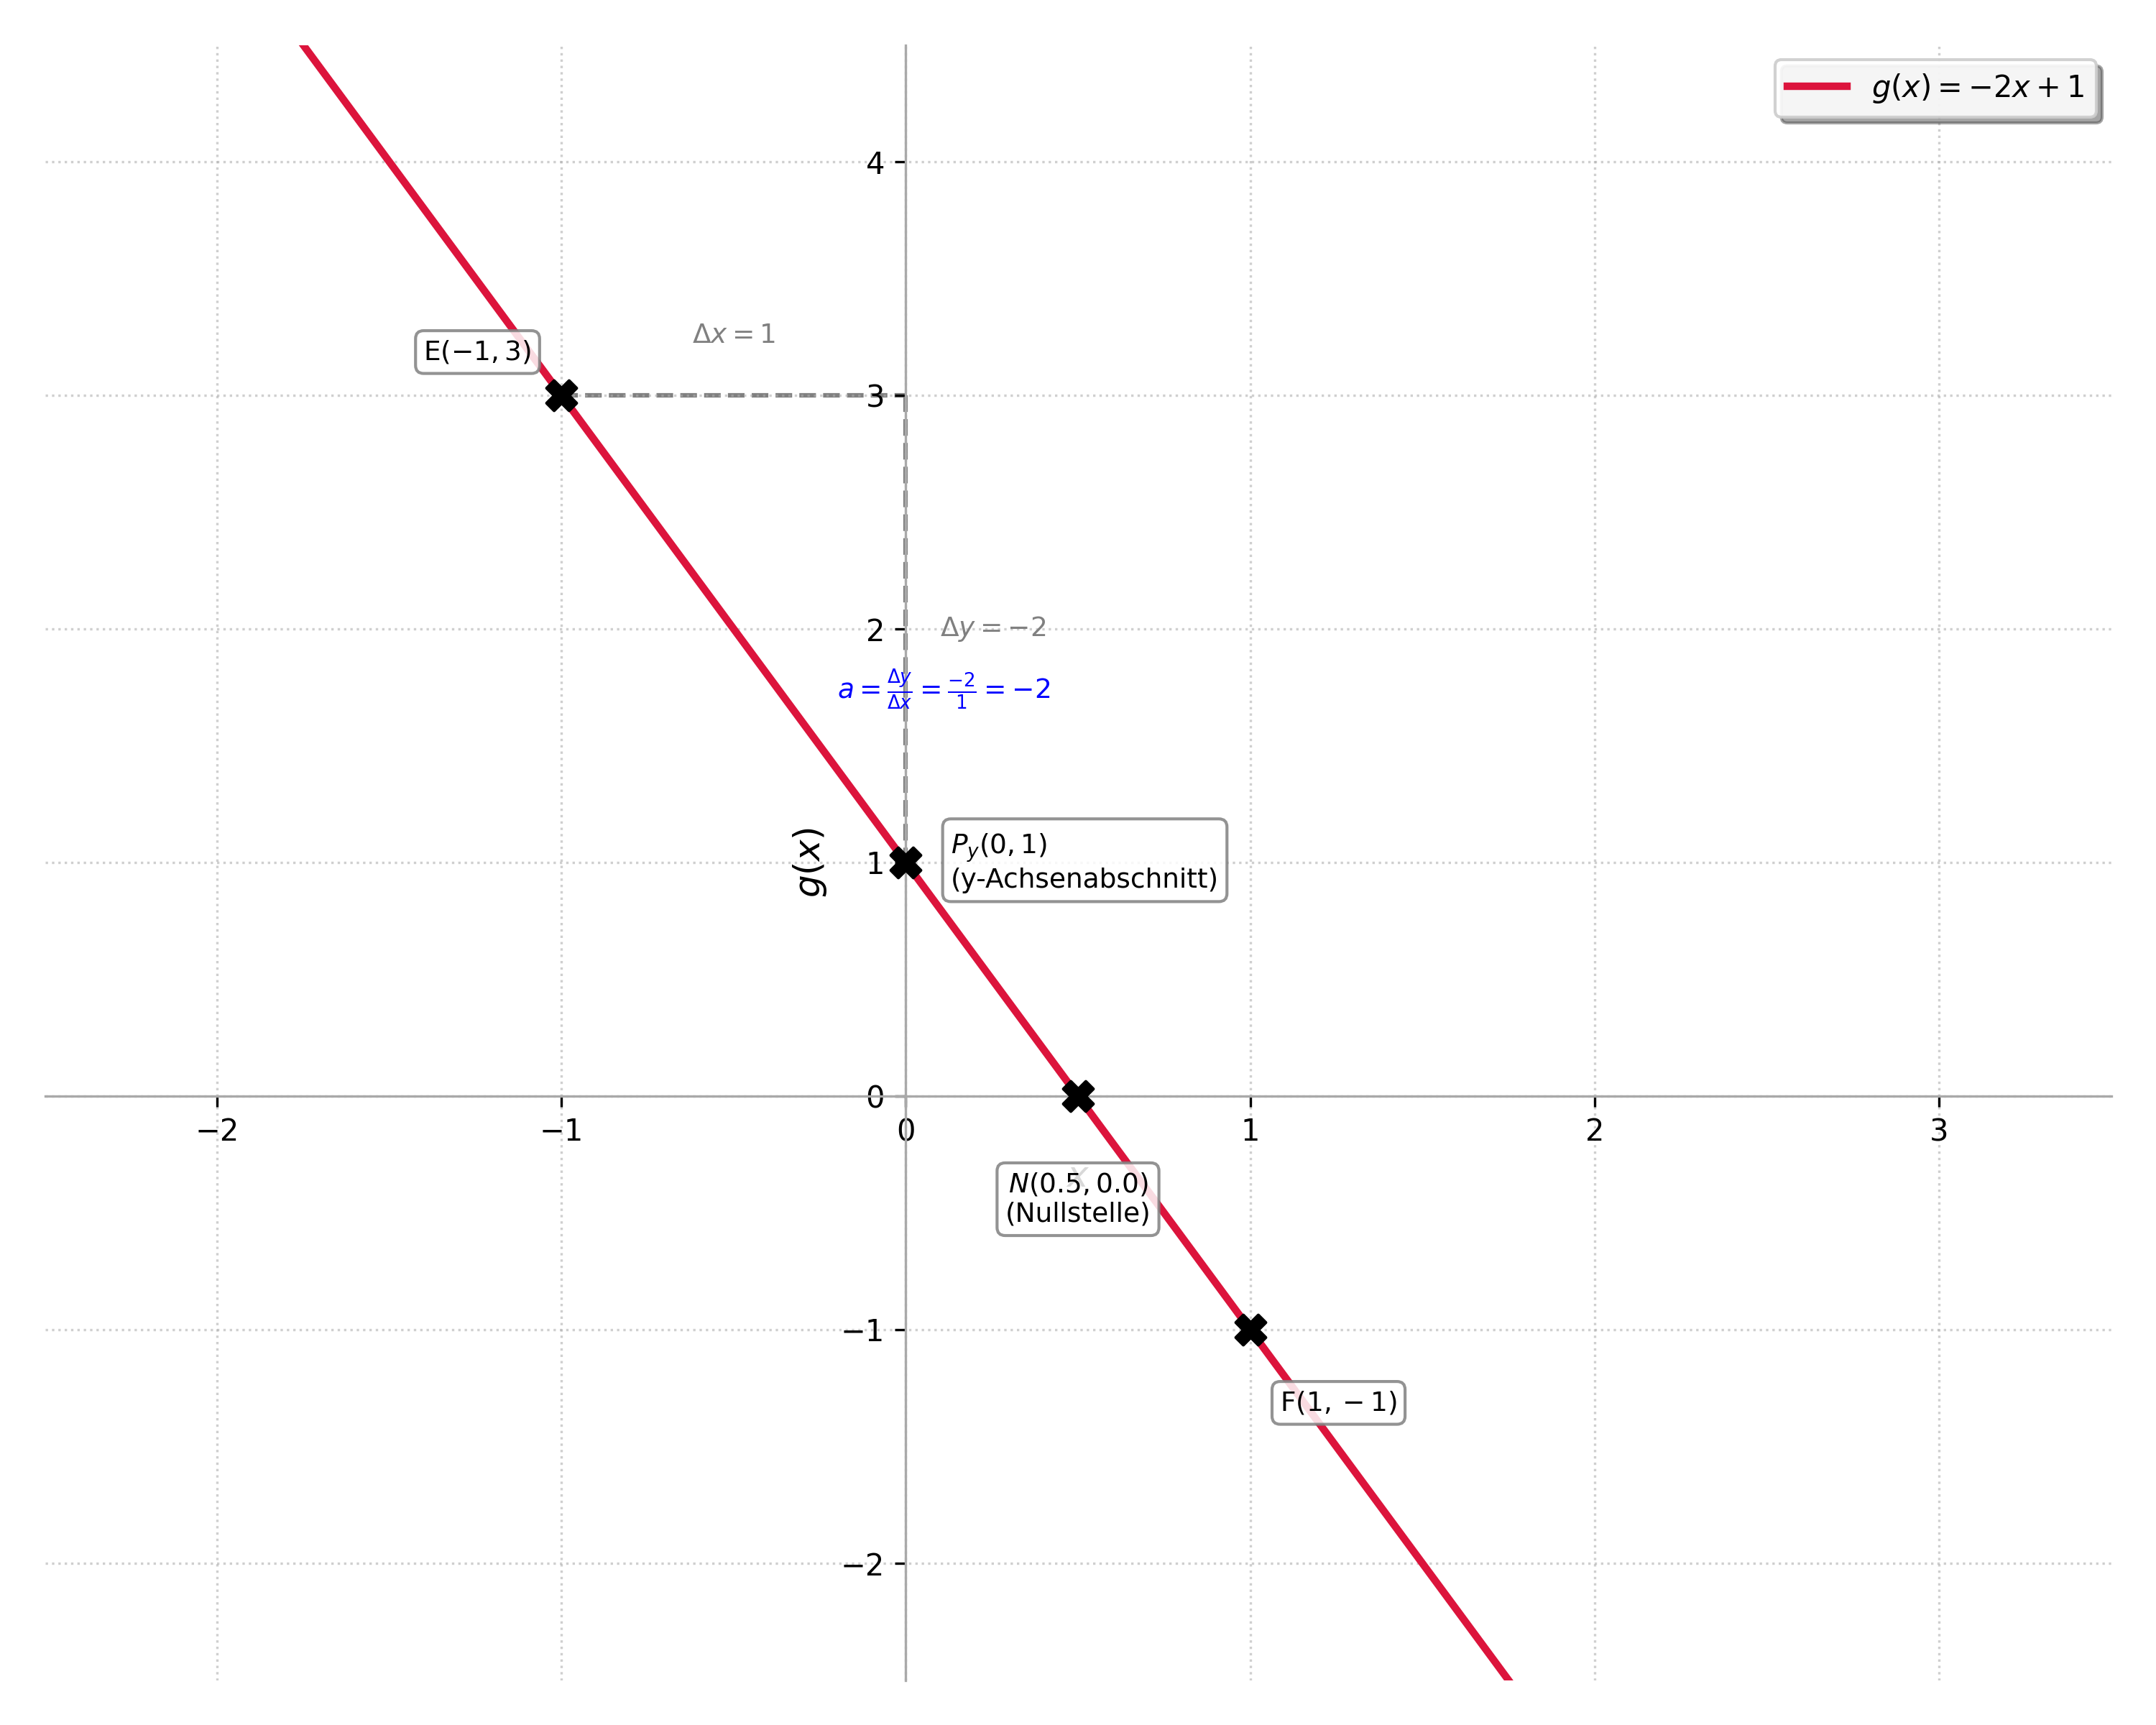
\includegraphics[width=0.8\textwidth]{grafiken/lin_fkt_teil2_skizze.png}
    % --- Beschreibung der Grafik für Teil 2 ---
    % Die Grafik sollte ein Koordinatensystem zeigen.
    % Eingezeichnet ist die Gerade g(x) = -2x + 1.
    % Die Punkte E(-1|3) und F(1|-1) sind markiert.
    % Der y-Achsenabschnitt (0|1) ist markiert.
    % Die Nullstelle (0.5|0) ist markiert.
    % Ein Steigungsdreieck ist eingezeichnet, das die Steigung a=-2 verdeutlicht (z.B. von E aus: 1 Einheit nach rechts, 2 Einheiten nach unten).
    % Die Achsen sind beschriftet (x und y oder g(x)).
    \captionof{figure}{Skizze der Funktion $g(x)=-2x+1$ mit Punkten E und F, y-Achsenabschnitt und Nullstelle.}
    \label{fig:lin_fkt_teil2}
    \end{center}
    \textbf{Überprüfung anhand der Skizze:} Man sollte erkennen, dass die Gerade durch die Punkte E und F verläuft und fallend ist ($a<0$). Der Schnittpunkt mit der y-Achse sollte bei $y=1$ liegen. Die Nullstelle sollte bei $x=0.5$ liegen. Das Steigungsdreieck sollte eine Steigung von $a=-2$ (z.B. 1 Einheit nach rechts, 2 Einheiten nach unten) visuell bestätigen.

    \item \textbf{Vorzeichen der Funktionswerte:}
    Die Nullstelle ist $x_N = \frac{1}{2}$ und die Steigung ist $a=-2$ (negativ).
    \begin{itemize}
        \item Für $x < x_N$ (also $x < \frac{1}{2}$): Die Funktionswerte $g(x)$ sind \textbf{positiv}. Da die Gerade fällt ($a<0$), kommt sie von 'oben links' und durchquert die x-Achse an der Nullstelle. Links von der Nullstelle liegen die Funktionswerte oberhalb der x-Achse. Z.B. $g(0) = 1$.
        \item Für $x > x_N$ (also $x > \frac{1}{2}$): Die Funktionswerte $g(x)$ sind \textbf{negativ}. Rechts von der Nullstelle liegen die Funktionswerte unterhalb der x-Achse. Z.B. $g(1) = -1$.
    \end{itemize}
\end{enumerate}

\end{loesungsumgebung}

\begin{aufgabenumgebung}{Nullstellen finden}
Berechne die Nullstellen der folgenden linearen Funktionen. Gib auch den Schnittpunkt mit der x-Achse an.
\begin{enumerate}
    \item $f(x) = 3x + 6$
    \item $g(x) = -0.5x + 2$
    \item $h(x) = 4x$
    \item $k(x) = 5$ (Was passiert hier?)
\end{enumerate}
\end{aufgabenumgebung}

\begin{loesungsumgebung}[loes:nullstellen-finden-mit-umformung]{Nullstellen finden}
Die Nullstelle einer Funktion ist der $x$-Wert, an dem der Funktionswert $f(x)$ gleich Null ist. Grafisch entspricht dies der x-Koordinate des Schnittpunktes des Graphen mit der x-Achse. Um die Nullstelle(n) zu berechnen, setzen wir $f(x)=0$ und lösen die Gleichung nach $x$ auf. Der Schnittpunkt mit der x-Achse hat dann die Koordinaten $(x_N|0)$, wobei $x_N$ die Nullstelle ist.

\begin{enumerate}
    \item \textbf{Funktion $f(x) = 3x + 6$} \\
    Wir setzen $f(x)=0$. Die Umformungsschritte sind:
    $$
    \begin{array}{r c l c l}
    \umformung{3x+6}{0}{-}{6}
    \umformung{3x}{-6}{\div}{3}
    \umformungend{x}{-2}
    \end{array}
    $$
    Die Nullstelle ist $x_N = -2$. \\
    Der Schnittpunkt mit der x-Achse ist $S_x(-2|0)$.

    \item \textbf{Funktion $g(x) = -0.5x + 2$} \\
    Wir setzen $g(x)=0$. Die Umformungsschritte sind:
    $$
    \begin{array}{r c l c l}
    \umformung{-0.5x + 2}{0}{-}{2}
    \umformung{-0.5x}{-2}{\div}{(-0.5)}
    \umformungend{x}{4}
    \end{array}
    $$
    Die Nullstelle ist $x_N = 4$. \\
    Der Schnittpunkt mit der x-Achse ist $S_x(4|0)$.

    \item \textbf{Funktion $h(x) = 4x$} \\
    Wir setzen $h(x)=0$. Die Umformungsschritte sind:
    $$
    \begin{array}{r c l c l}
    \umformung{4x}{0}{\div}{4}
    \umformungend{x}{0}
    \end{array}
    $$
    Die Nullstelle ist $x_N = 0$. \\
    Der Schnittpunkt mit der x-Achse ist $S_x(0|0)$. Dieser Punkt ist auch der Ursprung des Koordinatensystems und gleichzeitig der y-Achsenabschnitt.

    \item \textbf{Funktion $k(x) = 5$} \\
    Wir setzen $k(x)=0$:
    $$ 5 = 0 $$
    \textbf{Was passiert hier?} Die Gleichung $5=0$ ist eine falsche Aussage. Das bedeutet, es gibt keinen $x$-Wert, für den $k(x)=0$ wird.
    \textbf{Erklärung:} Die Funktion $k(x)=5$ ist eine konstante Funktion. Ihr Graph ist eine horizontale Gerade, die parallel zur x-Achse im Abstand von 5 Einheiten verläuft (also durch den Punkt $(0|5)$). Da diese Gerade die x-Achse niemals schneidet (es sei denn, die Konstante wäre 0), hat die Funktion keine Nullstellen. \\
    Die Funktion $k(x)=5$ hat \textbf{keine Nullstellen}. Es gibt keinen Schnittpunkt mit der x-Achse.
\end{enumerate}

\begin{merksatzumgebung}{Nullstellen und konstante Funktionen}
\begin{itemize}
    \item Eine \textbf{Nullstelle} $x_N$ einer Funktion $f$ ist ein Wert im Definitionsbereich, für den $f(x_N)=0$ gilt. Der Punkt $(x_N|0)$ ist der Schnittpunkt des Graphen mit der x-Achse.
    \item Lineare Funktionen der Form $f(x) = ax+b$ mit $a \neq 0$ haben immer genau eine Nullstelle bei $x_N = -\frac{b}{a}$.
    \item Konstante Funktionen $f(x)=c$ (wobei $c$ eine Zahl ist):
    \begin{itemize}
        \item Wenn $c \neq 0$ (wie bei $k(x)=5$), hat die Funktion \textbf{keine Nullstellen}, da ihr Graph eine horizontale Linie ist, die die x-Achse nicht schneidet.
        \item Wenn $c = 0$ (also $f(x)=0$), dann ist jeder $x$-Wert eine Nullstelle, da der Graph der Funktion die x-Achse selbst ist. In diesem Fall hat die Funktion unendlich viele Nullstellen.
    \end{itemize}
\end{itemize}
\end{merksatzumgebung}

\end{loesungsumgebung}


\begin{aufgabenumgebung}{Deine Wertetabelle}
Erstelle eine Wertetabelle für die Funktion $g(x) = -2x + 3$ für die x-Werte von -3 bis 3 in Einerschritten. Zeichne anschließend den Graphen der Funktion mithilfe der Punkte aus deiner Wertetabelle.
\end{aufgabenumgebung}


\begin{loesungsumgebung}[loes:wertetabelle-zeichnen]{Deine Wertetabelle}
Um die Wertetabelle für die Funktion $g(x) = -2x + 3$ zu erstellen, setzen wir die gegebenen x-Werte (-3, -2, -1, 0, 1, 2, 3) nacheinander in die Funktionsgleichung ein und berechnen den jeweiligen Funktionswert $g(x)$.

\textbf{Schritt 1: Funktionswerte berechnen}
\begin{itemize}
    \item Für $x = -3$: $g(-3) = -2(-3) + 3 = 6 + 3 = 9$
    \item Für $x = -2$: $g(-2) = -2(-2) + 3 = 4 + 3 = 7$
    \item Für $x = -1$: $g(-1) = -2(-1) + 3 = 2 + 3 = 5$
    \item Für $x = 0$: $g(0) = -2(0) + 3 = 0 + 3 = 3$
    \item Für $x = 1$: $g(1) = -2(1) + 3 = -2 + 3 = 1$
    \item Für $x = 2$: $g(2) = -2(2) + 3 = -4 + 3 = -1$
    \item Für $x = 3$: $g(3) = -2(3) + 3 = -6 + 3 = -3$
\end{itemize}

\textbf{Schritt 2: Wertetabelle erstellen}
Die berechneten Wertepaare $(x | g(x))$ können wir nun in einer Tabelle zusammenfassen:

\begin{center}
\begin{tabular}{r r}
\toprule
\multicolumn{1}{c}{$x$} & \multicolumn{1}{c}{$g(x) = -2x + 3$} \\
\midrule
$-3$ & $9$ \\
$-2$ & $7$ \\
$-1$ & $5$ \\
$0$ & $3$ \\
$1$ & $1$ \\
$2$ & $-1$ \\
$3$ & $-3$ \\
\bottomrule
\end{tabular}
\end{center}

\textbf{Schritt 3: Graphen der Funktion zeichnen}
Mithilfe der Punkte aus der Wertetabelle $( (-3|9), (-2|7), (-1|5), (0|3), (1|1), (2|-1), (3|-3) )$ kann nun der Graph der Funktion $g(x) = -2x+3$ gezeichnet werden. Da es sich um eine lineare Funktion handelt, liegen alle Punkte auf einer Geraden.

\begin{center}
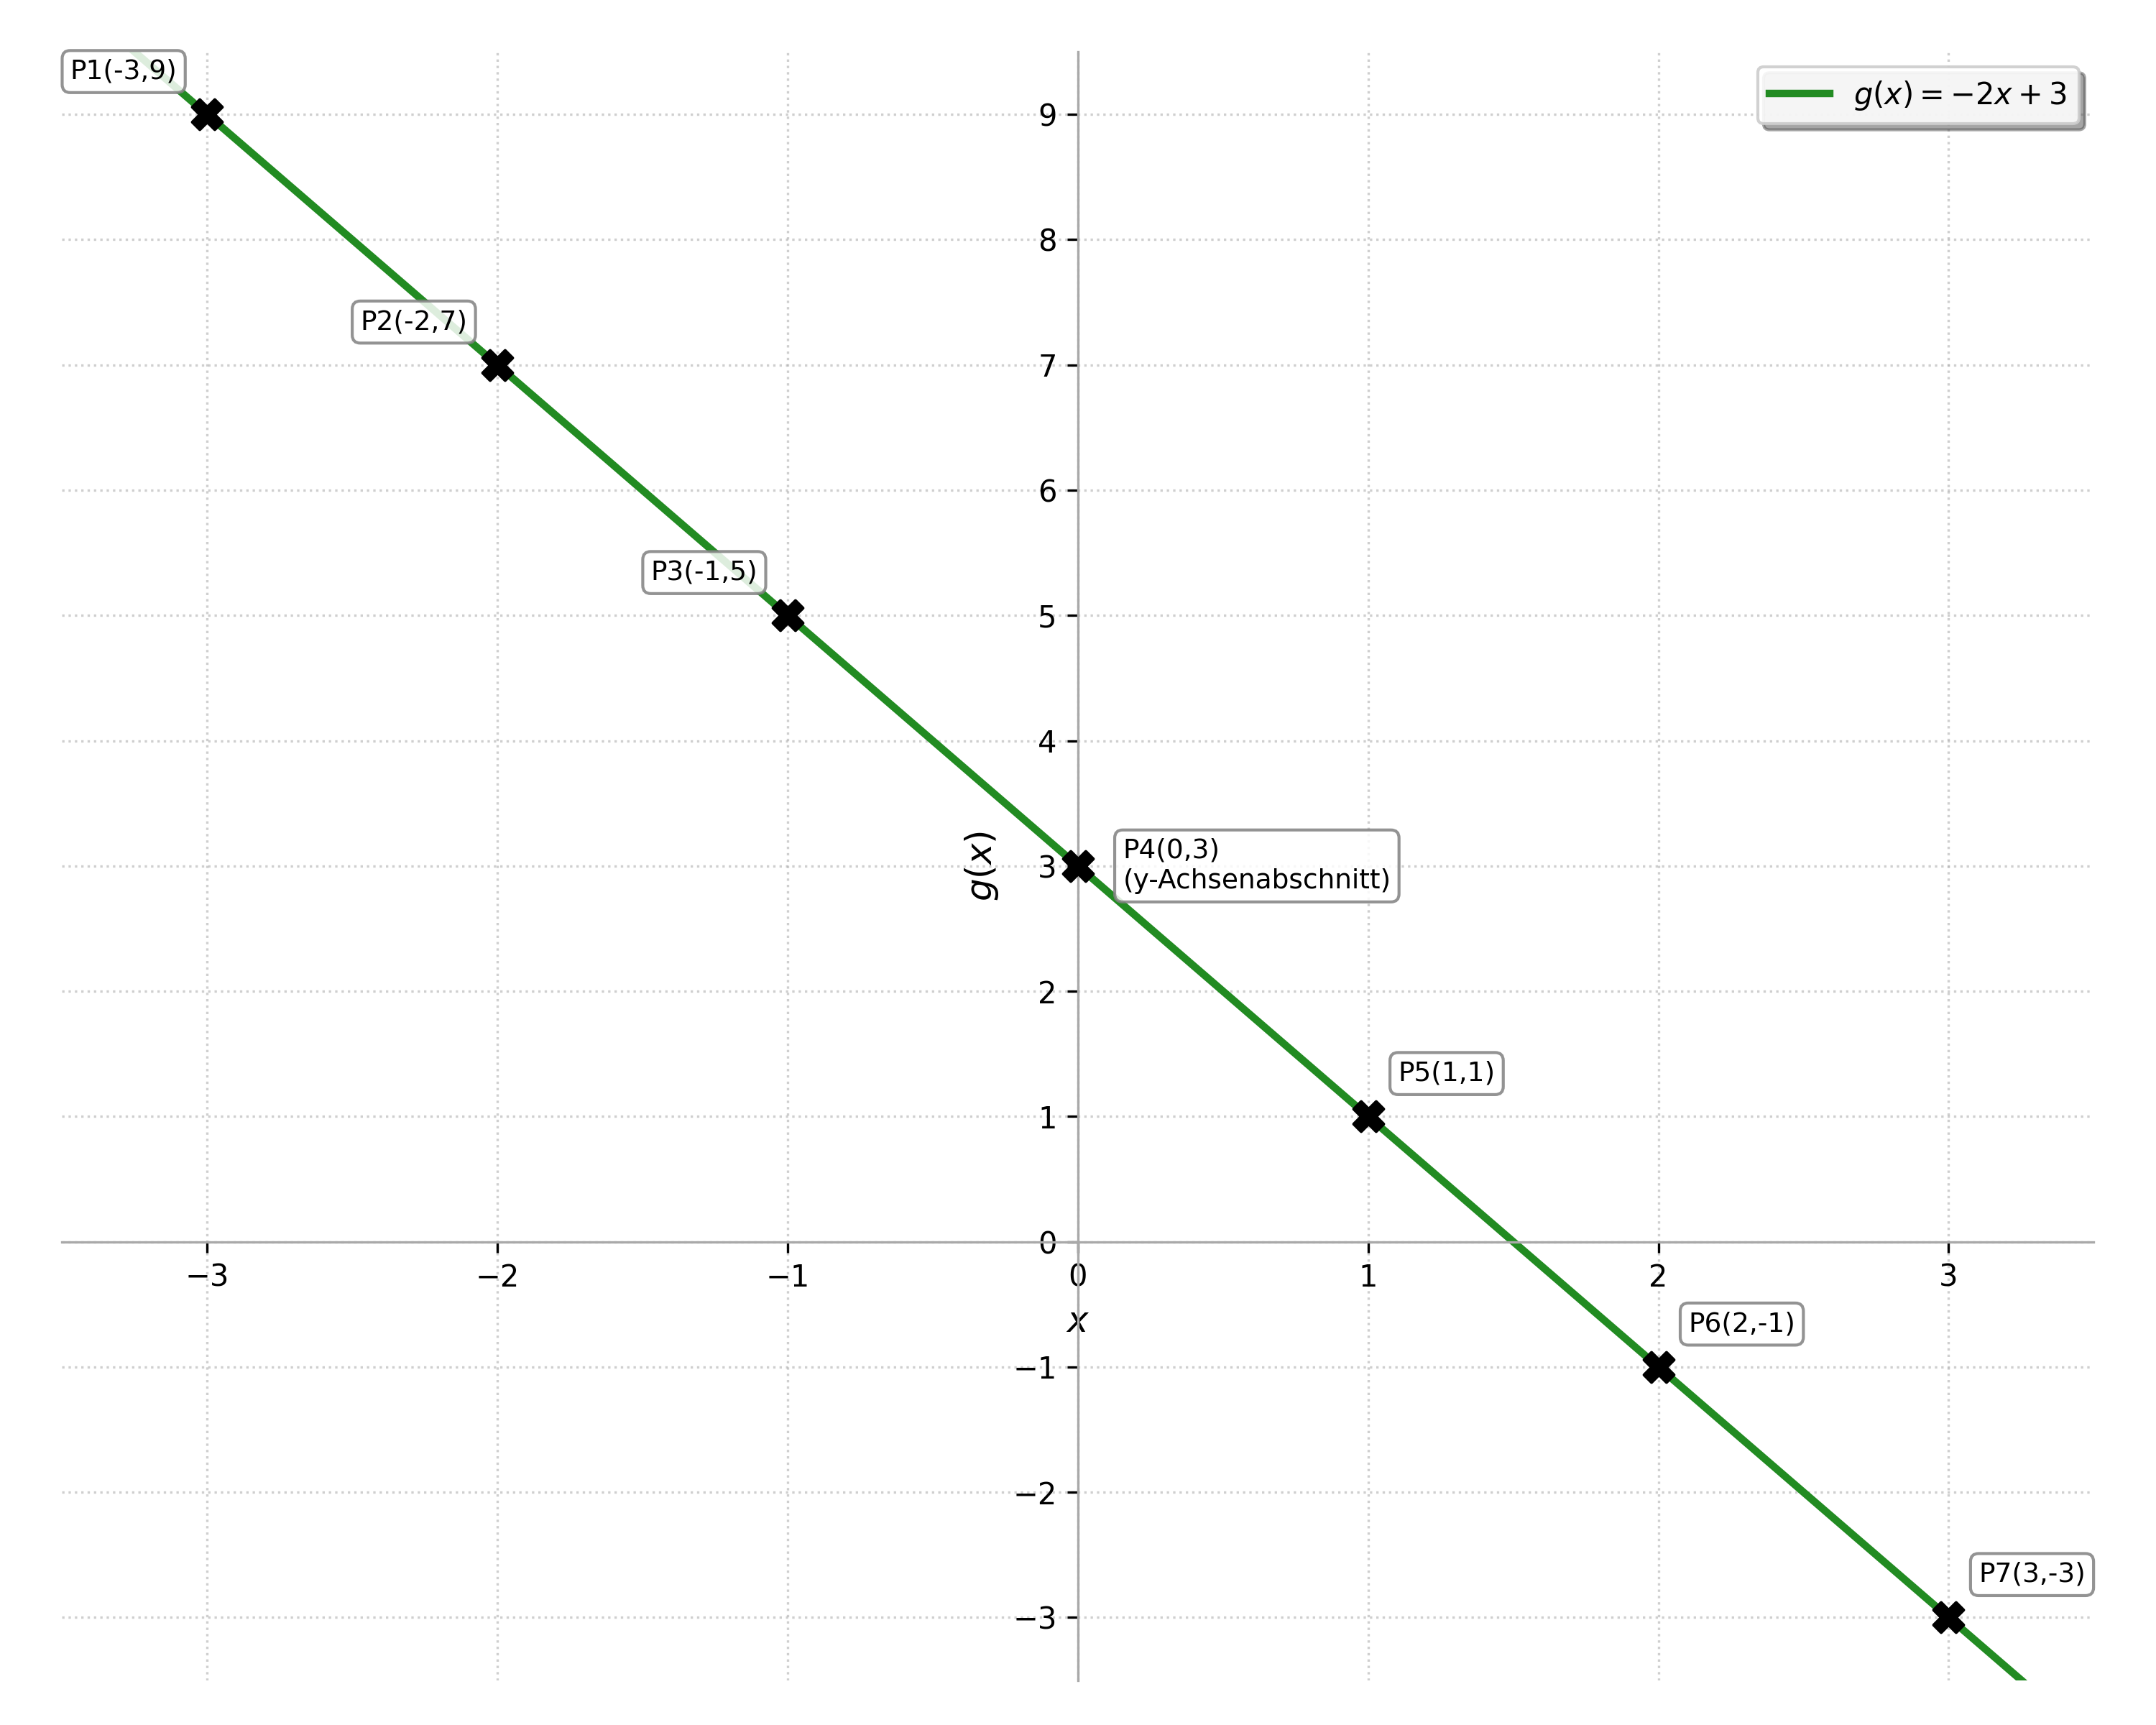
\includegraphics[width=0.8\textwidth]{grafiken/wertetabelle_graph_g_x.png}
% --- Beschreibung der Grafik ---
% Die Grafik sollte ein kartesisches Koordinatensystem zeigen (x-Achse und y-Achse bzw. g(x)-Achse).
% Die x-Achse sollte mindestens von -3 bis 3 skaliert sein.
% Die y-Achse sollte mindestens von -3 bis 9 skaliert sein.
% Die folgenden Punkte aus der Wertetabelle sind deutlich markiert:
% P1(-3|9), P2(-2|7), P3(-1|5), P4(0|3), P5(1|1), P6(2|-1), P7(3|-3).
% Eine Gerade ist durch diese Punkte gezeichnet. Diese Gerade ist der Graph von g(x) = -2x + 3.
% Die Gerade sollte fallend sein, da die Steigung -2 ist.
% Der Schnittpunkt mit der y-Achse bei (0|3) sollte erkennbar sein.
% Die Achsen sind beschriftet.
\captionof{figure}{Graph der Funktion $g(x) = -2x+3$ gezeichnet mit Punkten aus der Wertetabelle.}
\label{fig:graph_g_x}
\end{center}

\begin{tippumgebung}{Graph aus Wertetabelle zeichnen}
Wenn du Punkte aus einer Wertetabelle in ein Koordinatensystem einzeichnest:
\begin{itemize}
    \item Wähle eine passende Skalierung für die x- und y-Achse, damit alle Punkte gut sichtbar sind.
    \item Trage jeden Punkt $(x|y)$ sorgfältig ein: Gehe auf der x-Achse zum x-Wert und von dort parallel zur y-Achse zum y-Wert.
    \item Bei einer linearen Funktion müssen alle Punkte auf einer Geraden liegen. Du kannst ein Lineal verwenden, um dies zu überprüfen und die Gerade zu zeichnen.
    \item Der Punkt $(0|g(0))$ ist immer der Schnittpunkt mit der y-Achse. In diesem Fall $(0|3)$.
\end{itemize}
\end{tippumgebung}

\end{loesungsumgebung}



\begin{aufgabenumgebung}{Umgang mit linearen Funktionen: Werte und Schnittpunkte}

\textbf{Teil 1: Funktion $f(x) = -3x + 7$} \\
Gegeben ist die Funktion $f(x) = -3x + 7$.
\begin{enumerate}[label=(\alph*)]
    \item Berechne $f(-2)$, $f(0)$ und $f(4)$.
    \item Für welchen Wert von $x$ gilt $f(x) = 10$?
    \item Für welchen Wert von $x$ gilt $f(x) = -5$?
    \item An welcher Stelle schneidet der Graph die y-Achse? An welcher die x-Achse (Nullstelle)?
\end{enumerate}

\bigskip % Fügt einen größeren vertikalen Abstand ein

\textbf{Teil 2: Funktion $g(x) = \frac{1}{2}x - 1$} \\
Gegeben ist die Funktion $g(x) = \frac{1}{2}x - 1$.
\begin{enumerate}[label=(\alph*)]
    \item Berechne $g(-4)$, $g(0)$ und $g(6)$.
    \item Für welchen Wert von $x$ gilt $g(x) = 3$?
    \item Für welchen Wert von $x$ gilt $g(x) = -2.5$?
    \item An welcher Stelle schneidet der Graph die y-Achse? An welcher die x-Achse (Nullstelle)?
\end{enumerate}

\bigskip % Fügt einen größeren vertikalen Abstand ein

\textbf{Teil 3: Funktion $h(x) = -4x$} \\
Gegeben ist die Funktion $h(x) = -4x$.
\begin{enumerate}[label=(\alph*)]
    \item Berechne $h(-1.5)$, $h(0)$ und $h(2.5)$.
    \item Für welchen Wert von $x$ gilt $h(x) = 12$?
    \item Für welchen Wert von $x$ gilt $h(x) = -1$?
    \item An welcher Stelle schneidet der Graph die y-Achse? An welcher die x-Achse (Nullstelle)? Was ist hier besonders?
\end{enumerate}
\end{aufgabenumgebung}


\begin{loesungsumgebung}[loes:werte-und-schnittpunkte]{Umgang mit linearen Funktionen: Werte und Schnittpunkte}

\subsection*{Teil 1: Funktion $f(x) = -3x + 7$}
Gegeben ist die Funktion $f(x) = -3x + 7$.

\begin{enumerate}[label=(\alph*)]
    \item \textbf{Berechne $f(-2)$, $f(0)$ und $f(4)$.}
    \begin{itemize}
        \item $f(-2) = -3(-2) + 7 = 6 + 7 = 13$
        \item $f(0) = -3(0) + 7 = 0 + 7 = 7$
        \item $f(4) = -3(4) + 7 = -12 + 7 = -5$
    \end{itemize}

    \item \textbf{Für welchen Wert von $x$ gilt $f(x) = 10$?} \\
    Wir setzen $f(x) = 10$:
    $$
    \begin{array}{r c l c l}
    \umformung{-3x + 7}{10}{-}{7}
    \umformung{-3x}{3}{\div}{(-3)}
    \umformungend{x}{-1}
    \end{array}
    $$
    Für $x=-1$ gilt $f(x)=10$.

    \item \textbf{Für welchen Wert von $x$ gilt $f(x) = -5$?} \\
    Wir setzen $f(x) = -5$:
    $$
    \begin{array}{r c l c l}
    \umformung{-3x + 7}{-5}{-}{7}
    \umformung{-3x}{-12}{\div}{(-3)}
    \umformungend{x}{4}
    \end{array}
    $$
    Für $x=4$ gilt $f(x)=-5$.

    \item \textbf{An welcher Stelle schneidet der Graph die y-Achse? An welcher die x-Achse (Nullstelle)?}
    \begin{itemize}
        \item \textbf{Schnittpunkt mit der y-Achse:} \\
        Dieser liegt bei $x=0$. Der y-Wert ist $f(0) = -3(0) + 7 = 7$. \\
        Der Graph schneidet die y-Achse im Punkt $S_y(0|7)$.
        \item \textbf{Schnittpunkt mit der x-Achse (Nullstelle):} \\
        Wir setzen $f(x)=0$:
        $$
        \begin{array}{r c l c l}
        \umformung{-3x + 7}{0}{-}{7}
        \umformung{-3x}{-7}{\div}{(-3)}
        \umformungend{x}{\frac{7}{3}}
        \end{array}
        $$
        Die Nullstelle ist $x_N = \frac{7}{3}$. \\
        Der Graph schneidet die x-Achse im Punkt $S_x\left(\frac{7}{3}|0\right)$.
    \end{itemize}
\end{enumerate}

\bigskip % Fügt einen größeren vertikalen Abstand ein

\subsection*{Teil 2: Funktion $g(x) = \frac{1}{2}x - 1$}
Gegeben ist die Funktion $g(x) = \frac{1}{2}x - 1$.

\begin{enumerate}[label=(\alph*)]
    \item \textbf{Berechne $g(-4)$, $g(0)$ und $g(6)$.}
    \begin{itemize}
        \item $g(-4) = \frac{1}{2}(-4) - 1 = -2 - 1 = -3$
        \item $g(0) = \frac{1}{2}(0) - 1 = 0 - 1 = -1$
        \item $g(6) = \frac{1}{2}(6) - 1 = 3 - 1 = 2$
    \end{itemize}

    \item \textbf{Für welchen Wert von $x$ gilt $g(x) = 3$?} \\
    Wir setzen $g(x)=3$:
    $$
    \begin{array}{r c l c l}
    \umformung{\frac{1}{2}x - 1}{3}{+}{1}
    \umformung{\frac{1}{2}x}{4}{\cdot}{2}
    \umformungend{x}{8}
    \end{array}
    $$
    Für $x=8$ gilt $g(x)=3$.

    \item \textbf{Für welchen Wert von $x$ gilt $g(x) = -2.5$?} \\
    Wir setzen $g(x)=-2.5$:
    $$
    \begin{array}{r c l c l}
    \umformung{\frac{1}{2}x - 1}{-2.5}{+}{1}
    \umformung{\frac{1}{2}x}{-1.5}{\cdot}{2}
    \umformungend{x}{-3}
    \end{array}
    $$
    Für $x=-3$ gilt $g(x)=-2.5$.

    \item \textbf{An welcher Stelle schneidet der Graph die y-Achse? An welcher die x-Achse (Nullstelle)?}
    \begin{itemize}
        \item \textbf{Schnittpunkt mit der y-Achse:} \\
        Dieser liegt bei $x=0$. Der y-Wert ist $g(0) = \frac{1}{2}(0) - 1 = -1$. \\
        Der Graph schneidet die y-Achse im Punkt $S_y(0|-1)$.
        \item \textbf{Schnittpunkt mit der x-Achse (Nullstelle):} \\
        Wir setzen $g(x)=0$:
        $$
        \begin{array}{r c l c l}
        \umformung{\frac{1}{2}x - 1}{0}{+}{1}
        \umformung{\frac{1}{2}x}{1}{\cdot}{2}
        \umformungend{x}{2}
        \end{array}
        $$
        Die Nullstelle ist $x_N = 2$. \\
        Der Graph schneidet die x-Achse im Punkt $S_x(2|0)$.
    \end{itemize}
\end{enumerate}

\bigskip % Fügt einen größeren vertikalen Abstand ein

\subsection*{Teil 3: Funktion $h(x) = -4x$}
Gegeben ist die Funktion $h(x) = -4x$.

\begin{enumerate}[label=(\alph*)]
    \item \textbf{Berechne $h(-1.5)$, $h(0)$ und $h(2.5)$.}
    \begin{itemize}
        \item $h(-1.5) = -4(-1.5) = 6$
        \item $h(0) = -4(0) = 0$
        \item $h(2.5) = -4(2.5) = -10$
    \end{itemize}

    \item \textbf{Für welchen Wert von $x$ gilt $h(x) = 12$?} \\
    Wir setzen $h(x)=12$:
    $$
    \begin{array}{r c l c l}
    \umformung{-4x}{12}{\div}{(-4)}
    \umformungend{x}{-3}
    \end{array}
    $$
    Für $x=-3$ gilt $h(x)=12$.

    \item \textbf{Für welchen Wert von $x$ gilt $h(x) = -1$?} \\
    Wir setzen $h(x)=-1$:
    $$
    \begin{array}{r c l c l}
    \umformung{-4x}{-1}{\div}{(-4)}
    \umformungend{x}{\frac{1}{4}} % oder 0.25
    \end{array}
    $$
    Für $x=\frac{1}{4}$ (oder $x=0.25$) gilt $h(x)=-1$.

    \item \textbf{An welcher Stelle schneidet der Graph die y-Achse? An welcher die x-Achse (Nullstelle)? Was ist hier besonders?}
    \begin{itemize}
        \item \textbf{Schnittpunkt mit der y-Achse:} \\
        Dieser liegt bei $x=0$. Der y-Wert ist $h(0) = -4(0) = 0$. \\
        Der Graph schneidet die y-Achse im Punkt $S_y(0|0)$.
        \item \textbf{Schnittpunkt mit der x-Achse (Nullstelle):} \\
        Wir setzen $h(x)=0$:
        $$
        \begin{array}{r c l c l}
        \umformung{-4x}{0}{\div}{(-4)}
        \umformungend{x}{0}
        \end{array}
        $$
        Die Nullstelle ist $x_N = 0$. \\
        Der Graph schneidet die x-Achse im Punkt $S_x(0|0)$.
        \item \textbf{Was ist hier besonders?} \\
        Der Schnittpunkt mit der y-Achse $S_y(0|0)$ und der Schnittpunkt mit der x-Achse $S_x(0|0)$ sind identisch. Beide Schnittpunkte liegen im Ursprung des Koordinatensystems. Dies ist charakteristisch für proportionale Funktionen (lineare Funktionen ohne konstanten Term, d.h. $b=0$), deren Graphen immer durch den Ursprung verlaufen.
    \end{itemize}
\end{enumerate}

\end{loesungsumgebung}



\begin{aufgabenumgebung}{Schnittpunkte berechnen und zeichnen}
\begin{enumerate}
    \item Berechne den Schnittpunkt der folgenden Geradenpaare:
        \begin{itemize}
            \item $f(x) = x + 3$ und $g(x) = -2x + 9$
            \item $h(x) = 0.25x - 2$ und $k(x) = 0.25x + 1$ (Was stellst du hier fest? Wie liegen die Geraden zueinander?)
            \item $m(x) = \frac{1}{3}x + 1$ und $n(x) = -\frac{2}{3}x + 4$
        \end{itemize}
    \item Gegeben sind die Funktionen $f(x) = -x+5$ und $g(x) = 2x-1$.
        \begin{itemize}
            \item Berechne ihren Schnittpunkt $S$.
            \item Zeichne beide Geraden und ihren Schnittpunkt in ein Koordinatensystem.
        \end{itemize}
\end{enumerate}
\end{aufgabenumgebung}


\begin{loesungsumgebung}[loes:schnittpunkte-berechnen-zeichnen]{Schnittpunkte berechnen und zeichnen}

\begin{enumerate}
    \item \textbf{Berechnung der Schnittpunkte von Geradenpaaren:}
    Um den Schnittpunkt zweier Geraden $f(x)$ und $g(x)$ zu finden, setzt man die Funktionsterme gleich ($f(x)=g(x)$) und löst die entstehende Gleichung nach $x$ auf. Den gefundenen $x$-Wert setzt man dann in eine der ursprünglichen Geradengleichungen ein, um den zugehörigen $y$-Wert des Schnittpunktes $S(x|y)$ zu erhalten.

    \begin{itemize}
        \item \textbf{Geraden $f(x) = x + 3$ und $g(x) = -2x + 9$} \\
        Gleichsetzen: $f(x) = g(x)$
        $$ x + 3 = -2x + 9 $$
        Umformungsschritte:
        $$
        \begin{array}{r c l c l}
        \umformung{x+3}{-2x+9}{+}{2x}
        \umformung{3x+3}{9}{-}{3}
        \umformung{3x}{6}{\div}{3}
        \umformungend{x}{2}
        \end{array}
        $$
        Den $x$-Wert in $f(x)$ einsetzen (oder in $g(x)$):
        $f(2) = 2 + 3 = 5$.
        Der Schnittpunkt ist $S(2|5)$.

        \item \textbf{Geraden $h(x) = 0.25x - 2$ und $k(x) = 0.25x + 1$} \\
        Gleichsetzen: $h(x) = k(x)$
        $$ 0.25x - 2 = 0.25x + 1 $$
        Umformungsschritte:
        $$
        \begin{array}{r c l c l}
        \umformung{0.25x - 2}{0.25x + 1}{-}{0.25x}
        \umformungend{-2}{1} % Dies ist ein Widerspruch
        \end{array}
        $$
        \textbf{Was stellst du hier fest? Wie liegen die Geraden zueinander?} \\
        Die Gleichung $-2 = 1$ ist eine falsche Aussage (ein Widerspruch). Das bedeutet, dass es keinen $x$-Wert gibt, für den die beiden Funktionswerte gleich sind. Die Geraden haben keinen Schnittpunkt.
        Betrachtet man die Funktionsgleichungen, so stellt man fest, dass beide Geraden die gleiche Steigung $m=0.25$ haben, aber unterschiedliche y-Achsenabschnitte ($b_h = -2$ und $b_k = 1$). Geraden mit gleicher Steigung und unterschiedlichem y-Achsenabschnitt sind \textbf{parallel und verschieden (echt parallel)}. Sie schneiden sich daher nie.

        \item \textbf{Geraden $m(x) = \frac{1}{3}x + 1$ und $n(x) = -\frac{2}{3}x + 4$} \\
        Gleichsetzen: $m(x) = n(x)$
        $$ \frac{1}{3}x + 1 = -\frac{2}{3}x + 4 $$
        Umformungsschritte:
        $$
        \begin{array}{r c l c l}
        \umformung{\frac{1}{3}x + 1}{-\frac{2}{3}x + 4}{+}{\frac{2}{3}x}
        \umformung{x + 1}{4}{-}{1}
        \umformungend{x}{3}
        \end{array}
        $$
        Den $x$-Wert in $m(x)$ einsetzen (oder in $n(x)$):
        $m(3) = \frac{1}{3}(3) + 1 = 1 + 1 = 2$.
        Der Schnittpunkt ist $S(3|2)$.
    \end{itemize}

    \item \textbf{Gegeben sind die Funktionen $f(x) = -x+5$ und $g(x) = 2x-1$.}
    \begin{itemize}
        \item \textbf{Berechne ihren Schnittpunkt $S$.} \\
        Gleichsetzen: $f(x) = g(x)$
        $$ -x + 5 = 2x - 1 $$
        Umformungsschritte:
        $$
        \begin{array}{r c l c l}
        \umformung{-x+5}{2x-1}{-}{2x}
        \umformung{-3x+5}{-1}{-}{5}
        \umformung{-3x}{-6}{\div}{(-3)}
        \umformungend{x}{2}
        \end{array}
        $$
        Den $x$-Wert in $f(x)$ einsetzen (oder in $g(x)$):
        $f(2) = -(2) + 5 = -2 + 5 = 3$.
        Der Schnittpunkt ist $S(2|3)$.

        \item \textbf{Zeichne beide Geraden und ihren Schnittpunkt in ein Koordinatensystem.}
        \begin{center}
        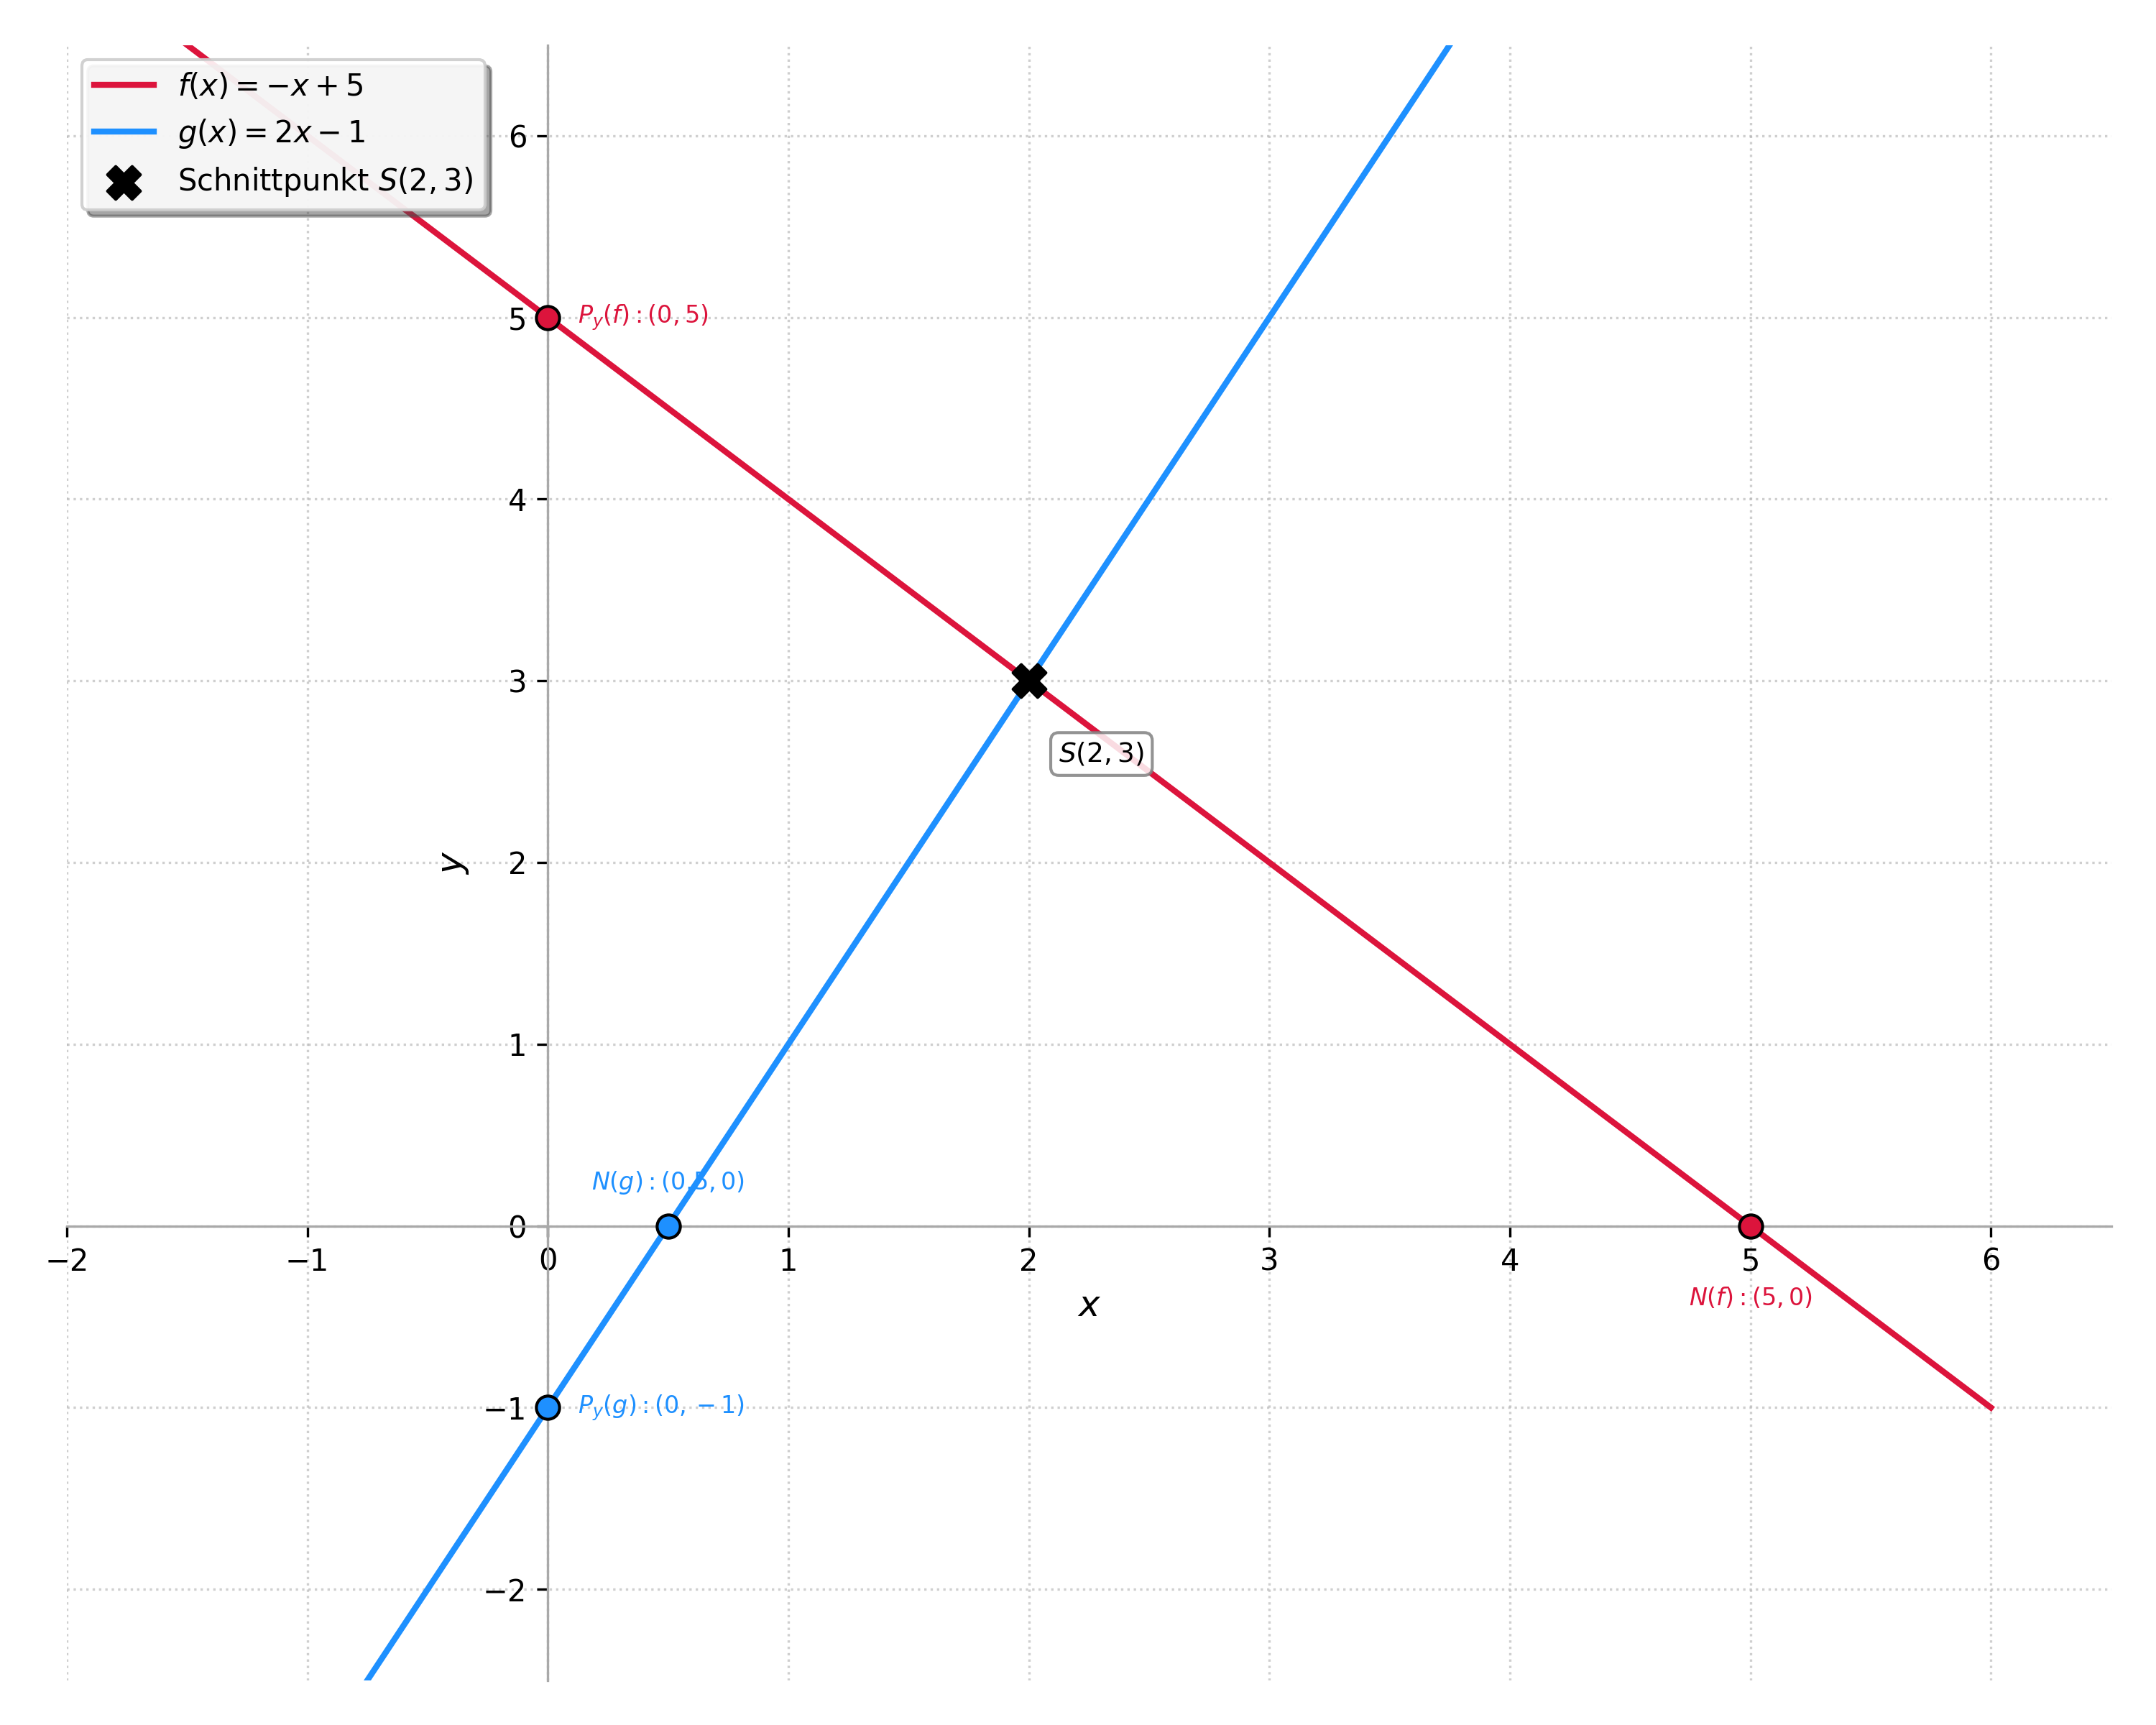
\includegraphics[width=0.8\textwidth]{grafiken/schnittpunkt_teil2_f_g.png}
        % --- Beschreibung der Grafik ---
        % Die Grafik sollte ein kartesisches Koordinatensystem zeigen.
        % Die x-Achse und y-Achse sind beschriftet und sinnvoll skaliert (z.B. von -2 bis 6 für x und -2 bis 6 für y).
        % Eingezeichnet sind die beiden Geraden:
        % 1. f(x) = -x + 5: y-Achsenabschnitt bei (0|5), Nullstelle bei (5|0). Die Gerade fällt.
        % 2. g(x) = 2x - 1: y-Achsenabschnitt bei (0|-1), Nullstelle bei (0.5|0). Die Gerade steigt.
        % Der berechnete Schnittpunkt S(2|3) ist deutlich markiert und liegt auf beiden Geraden.
        % Die Geraden könnten zur besseren Unterscheidung farblich oder durch Beschriftung (f(x), g(x)) gekennzeichnet sein.
        \captionof{figure}{Graphische Darstellung der Geraden $f(x) = -x+5$ und $g(x) = 2x-1$ mit ihrem Schnittpunkt $S(2|3)$.}
        \label{fig:schnittpunkt_f_g_teil2}
        \end{center}
    \end{itemize}
\end{enumerate}

\end{loesungsumgebung}

\begin{aufgabenumgebung}{Taxifahrt}
Ein Taxifahrer verlangt eine Grundgebühr von 3,50 Euro für jede Fahrt. Zusätzlich kostet jeder gefahrene Kilometer 2 Euro.
\begin{enumerate}
    \item Stelle die Kostenfunktion $K(x)$ auf, wobei $x$ die Anzahl der gefahrenen Kilometer ist. Identifiziere $a$ und $b$ und erkläre ihre Bedeutung in diesem Kontext.
    \item Wie viel kostet eine Fahrt von 15 km?
    \item Du hast 25 Euro dabei. Wie viele Kilometer kannst du maximal fahren, wenn du den vollen Betrag ausgeben möchtest? (Tipp: Setze $K(x)=25$ und löse die Gleichung nach $x$ auf.)
    \item Zeichne den Graphen der Funktion $K(x)$ für $x$-Werte von 0 km bis 20 km. Wähle passende Einheiten für die Achsen.
\end{enumerate}
\end{aufgabenumgebung}


\begin{loesungsumgebung}[loes:taxifahrt]{Taxifahrt}
Die Kosten für eine Taxifahrt setzen sich aus einer festen Grundgebühr und einem variablen Preis pro Kilometer zusammen. Dies lässt sich mathematisch durch eine lineare Funktion modellieren.

\begin{enumerate}
    \item \textbf{Kostenfunktion $K(x)$ aufstellen} \\
    Die allgemeine Form einer linearen Funktion ist $f(x) = ax + b$. In diesem Kontext ist:
    \begin{itemize}
        \item $x$: die Anzahl der gefahrenen Kilometer.
        \item $b$: die Grundgebühr, die unabhängig von der Strecke anfällt. Hier beträgt sie 3,50 Euro.
        \item $a$: die Kosten pro gefahrenem Kilometer. Hier sind es 2 Euro pro Kilometer.
    \end{itemize}
    Somit lautet die Kostenfunktion $K(x)$:
    $$ K(x) = 2x + 3.50 $$
    Identifikation und Bedeutung von $a$ und $b$:
    \begin{itemize}
        \item $a = 2$ (Euro/km): Dies ist die \textbf{Steigung} der Geraden. Sie gibt an, um wie viel sich die Gesamtkosten erhöhen, wenn ein zusätzlicher Kilometer gefahren wird. Jeder weitere Kilometer kostet also 2 Euro mehr.
        \item $b = 3.50$ (Euro): Dies ist der \textbf{y-Achsenabschnitt} der Geraden. Er repräsentiert die Fixkosten, also die Grundgebühr, die auch dann anfällt, wenn keine Kilometer gefahren werden ($x=0$). Es sind die Kosten für das Antreten der Fahrt.
    \end{itemize}

    \item \textbf{Wie viel kostet eine Fahrt von 15 km?} \\
    Wir setzen $x=15$ in die Kostenfunktion $K(x)$ ein:
    $$ K(15) = 2 \cdot (15) + 3.50 $$
    $$ K(15) = 30 + 3.50 $$
    $$ K(15) = 33.50 $$
    Eine Fahrt von 15 km kostet 33,50 Euro.

    \item \textbf{Wie viele Kilometer kannst du maximal fahren, wenn du 25 Euro dabei hast?} \\
    Wir setzen $K(x) = 25$ und lösen die Gleichung nach $x$ auf:
    $$ 2x + 3.50 = 25 $$
    Umformungsschritte:
    $$
    \begin{array}{r c l c l}
    \umformung{2x + 3.50}{25}{-}{3.50}
    \umformung{2x}{21.50}{\div}{2}
    \umformungend{x}{10.75}
    \end{array}
    $$
    Du kannst maximal 10,75 Kilometer fahren.

    \item \textbf{Zeichne den Graphen der Funktion $K(x)$ für $x$-Werte von 0 km bis 20 km.}
    \begin{center}
    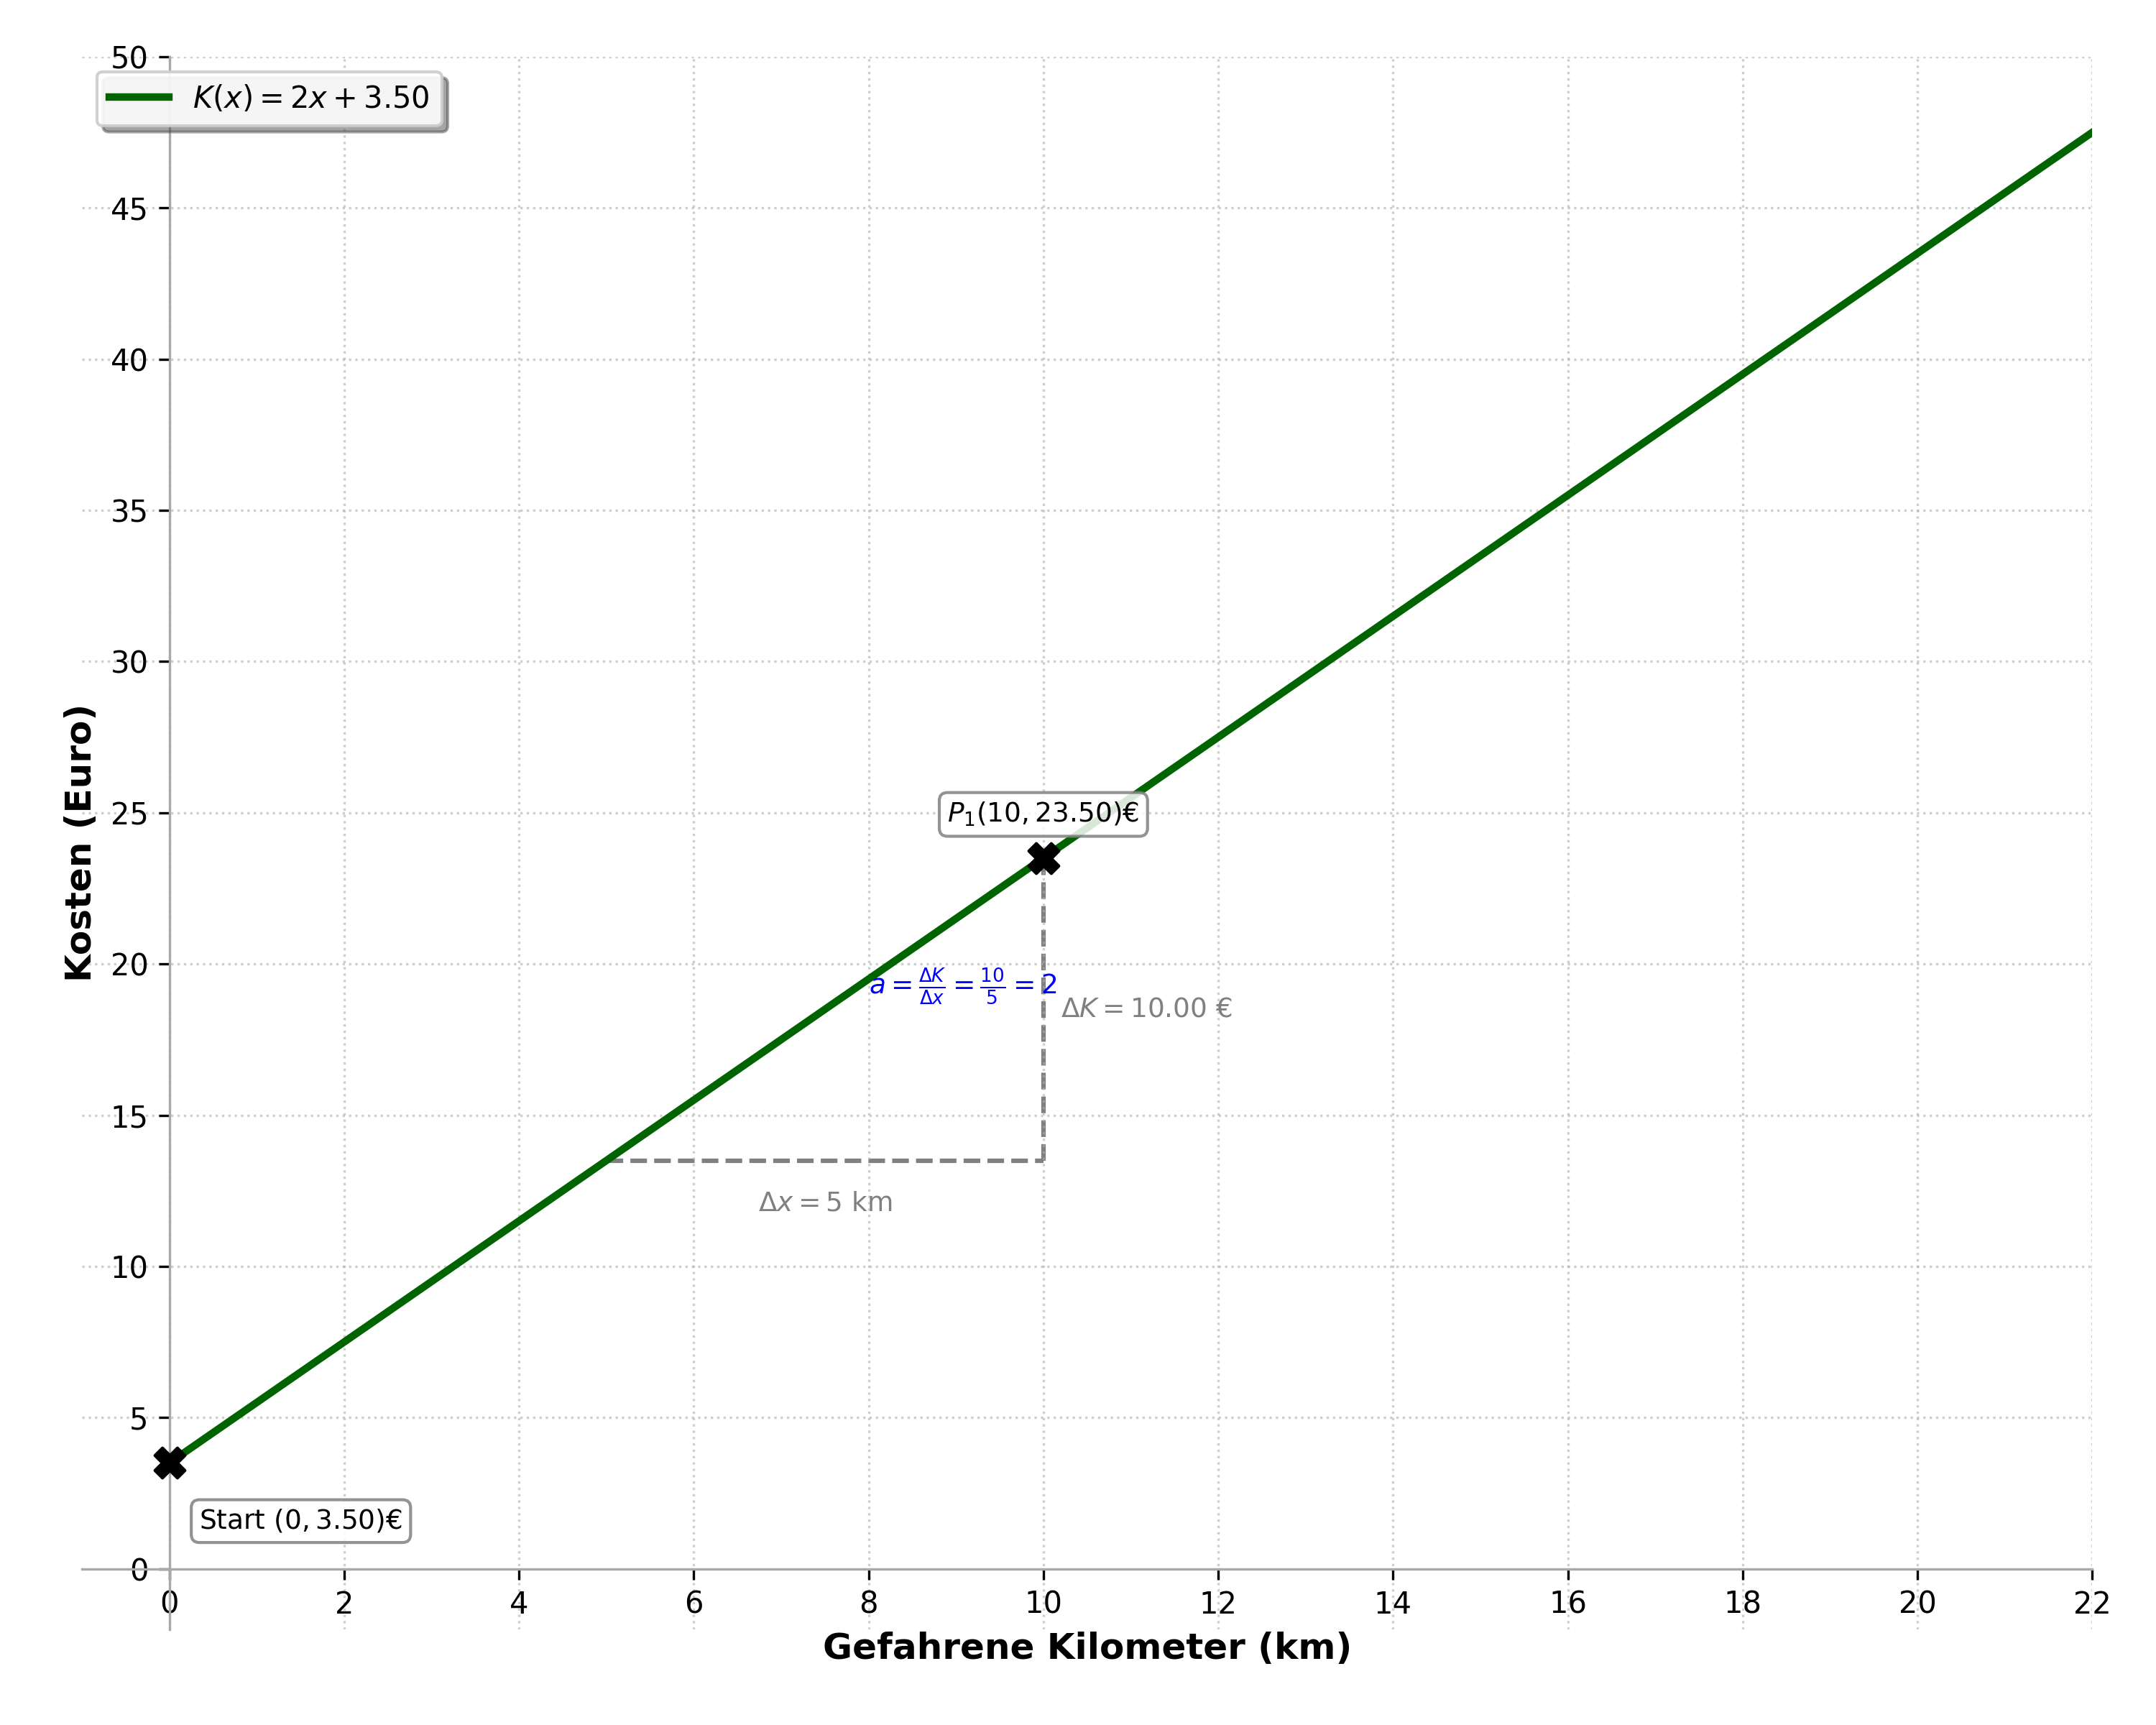
\includegraphics[width=0.8\textwidth]{grafiken/taxikosten_graph.png}
    % --- Beschreibung der Grafik ---
    % Die Grafik sollte ein kartesisches Koordinatensystem zeigen.
    % Die x-Achse ist mit 'Gefahrene Kilometer (km)' beschriftet und reicht von 0 bis mindestens 20 km.
    % Die y-Achse ist mit 'Kosten (Euro)' beschriftet und reicht von 0 bis ca. 45-50 Euro (da K(20) = 2*20 + 3.50 = 43.50 Euro).
    % Der Graph der Funktion K(x) = 2x + 3.50 ist als Gerade eingezeichnet, die bei x=0 beginnt.
    % Wichtige Punkte sind markiert oder ablesbar:
    % - Der y-Achsenabschnitt (Startpunkt der Fahrtkosten) bei (0 | 3.50).
    % - Ein weiterer Punkt, z.B. (10 | 23.50) oder der Endpunkt (20 | 43.50).
    % - Die Steigung von 2 (pro 1 km nach rechts geht es 2 Euro nach oben) sollte aus dem Graphen ersichtlich sein (z.B. durch ein Steigungsdreieck).
    \captionof{figure}{Graph der Kostenfunktion $K(x) = 2x + 3.50$ für eine Taxifahrt.}
    \label{fig:taxikosten}
    \end{center}
    \textbf{Erläuterung zur Zeichnung:}
    Der Graph beginnt auf der y-Achse beim Wert der Grundgebühr (3,50 Euro). Von dort steigt die Gerade linear an. Für jeden Kilometer, den man auf der x-Achse nach rechts geht, steigen die Kosten auf der y-Achse um 2 Euro. Für eine Strecke von 20 km würden die Kosten $K(20) = 2(20) + 3.50 = 43.50$ Euro betragen. Die Achsen sollten so skaliert sein, dass dieser Bereich gut dargestellt wird.
\end{enumerate}

\end{loesungsumgebung}

\begin{aufgabenumgebung}[labelA:LinUeb]{Lineare Funktionen – Übungen querbeet}
\begin{enumerate}
    \item \textbf{Paketversand:} Ein Paketversand kostet 5 Euro Grundgebühr. Jedes Kilogramm Gewicht kostet zusätzlich 1,50 Euro.
        \begin{itemize}
            \item Wie lautet die Kostenfunktion $K(g)$, wenn $g$ das Gewicht in Kilogramm ist?
            \item Was kostet ein Paket, das 3,2 kg wiegt?
            \item Ein Paket kostet 15,50 Euro. Wie schwer war es?
        \end{itemize}
    \item \textbf{Kerzenlänge:} Eine Kerze ist anfangs 20 cm lang. Pro Stunde brennt sie gleichmäßig 2,5 cm ab.
        \begin{itemize}
            \item Stelle eine Funktion $L(t)$ auf, die die Länge der Kerze nach $t$ Stunden beschreibt. (Achtung: Die Länge nimmt ab. Was bedeutet das für das Vorzeichen der Steigung $a$?)
            \item Wie lang ist die Kerze nach 3 Stunden?
            \item Nach wie vielen Stunden ist die Kerze komplett abgebrannt? (Das bedeutet, ihre Länge ist 0 cm.)
            \item Für welchen Zeitraum $t$ ist diese Funktion realistisch? (Definitionsbereich der Anwendung)
        \end{itemize}
    \item \textbf{Funktion aus Punkten:} Eine Gerade geht durch die Punkte $P_1(2|5)$ und $P_2(5|14)$. Bestimme ihre Funktionsgleichung $f(x)=ax+b$.
    \item \textbf{Funktion aus Steigung und Punkt:} Die Steigung einer Geraden ist $a = -2$. Die Gerade geht außerdem durch den Punkt $P(1|3)$. Bestimme den y-Achsenabschnitt $b$ und gib die vollständige Funktionsgleichung an. (Tipp: Setze $a$ und die Koordinaten von $P$ in $y=ax+b$ ein und löse nach $b$.)
\end{enumerate}
\end{aufgabenumgebung}


\begin{loesungsumgebung}[loes:LinUeb]{Lineare Funktionen – Übungen querbeet}

\begin{enumerate}
    \item \textbf{Paketversand:}
    \begin{itemize}
        \item \textbf{Wie lautet die Kostenfunktion $K(g)$, wenn $g$ das Gewicht in Kilogramm ist?} \\
        Die Grundgebühr beträgt 5 Euro (das ist der y-Achsenabschnitt $b$).
        Jedes Kilogramm kostet zusätzlich 1,50 Euro (das ist die Steigung $a$).
        Die Kostenfunktion lautet: $K(g) = 1.50g + 5$.

        \item \textbf{Was kostet ein Paket, das 3,2 kg wiegt?} \\
        Wir setzen $g = 3.2$ in die Funktion $K(g)$ ein:
        $K(3.2) = 1.50 \cdot (3.2) + 5 = 4.80 + 5 = 9.80$. \\
        Ein Paket, das 3,2 kg wiegt, kostet 9,80 Euro.

        \item \textbf{Ein Paket kostet 15,50 Euro. Wie schwer war es?} \\
        Wir setzen $K(g) = 15.50$ und lösen nach $g$ auf:
        $$ 1.50g + 5 = 15.50 $$
        Umformungsschritte:
        $$
        \begin{array}{r c l c l}
        \umformung{1.50g + 5}{15.50}{-}{5}
        \umformung{1.50g}{10.50}{\div}{1.50}
        \umformungend{g}{7}
        \end{array}
        $$
        Das Paket war 7 kg schwer.
    \end{itemize}

    \item \textbf{Kerzenlänge:}
    \begin{itemize}
        \item \textbf{Stelle eine Funktion $L(t)$ auf, die die Länge der Kerze nach $t$ Stunden beschreibt.} \\
        Die Anfangslänge beträgt 20 cm (das ist der y-Achsenabschnitt $b$).
        Pro Stunde brennt sie 2,5 cm ab. Da die Länge abnimmt, ist die Steigung $a$ negativ: $a = -2.5$ cm/Stunde.
        Die Funktion für die Länge $L(t)$ nach $t$ Stunden lautet: $L(t) = -2.5t + 20$.

        \item \textbf{Wie lang ist die Kerze nach 3 Stunden?} \\
        Wir setzen $t = 3$ in die Funktion $L(t)$ ein:
        $L(3) = -2.5 \cdot (3) + 20 = -7.5 + 20 = 12.5$. \\
        Nach 3 Stunden ist die Kerze noch 12,5 cm lang.

        \item \textbf{Nach wie vielen Stunden ist die Kerze komplett abgebrannt? (Länge ist 0 cm)} \\
        Wir setzen $L(t) = 0$ und lösen nach $t$ auf:
        $$ -2.5t + 20 = 0 $$
        Umformungsschritte:
        $$
        \begin{array}{r c l c l}
        \umformung{-2.5t + 20}{0}{-}{20}
        \umformung{-2.5t}{-20}{\div}{(-2.5)}
        \umformungend{t}{8}
        \end{array}
        $$
        Die Kerze ist nach 8 Stunden komplett abgebrannt.

        \item \textbf{Für welchen Zeitraum $t$ ist diese Funktion realistisch? (Definitionsbereich der Anwendung)} \\
        Die Zeit $t$ kann nicht negativ sein, also $t \ge 0$. Die Kerze kann nicht weiterbrennen, nachdem sie vollständig abgebrannt ist (nach 8 Stunden). Eine negative Länge ist nicht möglich.
        Daher ist der realistische Definitionsbereich für $t$ (in Stunden): $0 \le t \le 8$.
    \end{itemize}

    \item \textbf{Funktion aus Punkten:} Eine Gerade geht durch die Punkte $P_1(2|5)$ und $P_2(5|14)$. Bestimme ihre Funktionsgleichung $f(x)=ax+b$. \\
    \textbf{Schritt 1: Steigung $a$ berechnen}
    $$ a = \frac{y_2 - y_1}{x_2 - x_1} = \frac{14 - 5}{5 - 2} = \frac{9}{3} = 3 $$
    Die Steigung ist $a=3$.
    \textbf{Schritt 2: y-Achsenabschnitt $b$ berechnen}
    Wir verwenden die Form $f(x) = ax+b$, setzen $a=3$ und die Koordinaten eines Punktes (z.B. $P_1(2|5)$) ein: $x=2, y=5$.
    $$ 5 = 3 \cdot (2) + b $$
    $$ 5 = 6 + b $$
    Umformungsschritte (um $b$ zu isolieren, stellen wir $6+b=5$ um):
    $$
    \begin{array}{r c l c l}
    \umformung{6+b}{5}{-}{6}
    \umformungend{b}{-1}
    \end{array}
    $$
    Der y-Achsenabschnitt ist $b=-1$.
    \textbf{Schritt 3: Funktionsgleichung aufstellen}
    Die Funktionsgleichung lautet $f(x) = 3x - 1$.

    \item \textbf{Funktion aus Steigung und Punkt:} Die Steigung einer Geraden ist $a = -2$. Die Gerade geht außerdem durch den Punkt $P(1|3)$. Bestimme den y-Achsenabschnitt $b$ und gib die vollständige Funktionsgleichung an. \\
    Die allgemeine Form ist $y = ax+b$. Gegeben sind $a=-2$ und der Punkt $P(1|3)$, also $x=1$ und $y=3$.
    \textbf{Schritt 1: y-Achsenabschnitt $b$ berechnen}
    Wir setzen die gegebenen Werte in die Gleichung ein:
    $$ 3 = (-2) \cdot (1) + b $$
    $$ 3 = -2 + b $$
    Umformungsschritte (um $b$ zu isolieren, stellen wir $-2+b=3$ um):
    $$
    \begin{array}{r c l c l}
    \umformung{-2+b}{3}{+}{2}
    \umformungend{b}{5}
    \end{array}
    $$
    Der y-Achsenabschnitt ist $b=5$.
    \textbf{Schritt 2: Vollständige Funktionsgleichung angeben}
    Die Funktionsgleichung lautet $f(x) = -2x + 5$.
\end{enumerate}

\end{loesungsumgebung}

\begin{aufgabenumgebung}{Deine durchschnittliche Rate}
Denke dir ein eigenes Beispiel aus dem Alltag aus, bei dem eine Größe sich über die Zeit oder eine andere Einheit verändert (z.B. Wasserverbrauch einer Familie über mehrere Tage, Wachstum einer Pflanze über Wochen, Temperaturänderung im Laufe eines Tages, Anzahl der gelesenen Seiten eines Buches über mehrere Abende).
\begin{enumerate}
    \item Beschreibe die Situation klar. Welche Größe ändert sich in Abhängigkeit von welcher anderen Größe?
    \item Lege zwei Messpunkte (Anfangswert mit zugehörigem 'x1' und Endwert mit zugehörigem 'x2') fest.
    \item Berechne die durchschnittliche Änderungsrate. Was sagt diese Rate in deinem Beispiel konkret aus? Welche Einheit hat sie?
\end{enumerate}
\end{aufgabenumgebung}

\begin{loesungsumgebung}[loes:durchschnittliche-rate-beispiel]{Deine durchschnittliche Rate}
Hier ist ein Beispiel aus dem Alltag, das eine durchschnittliche Änderungsrate veranschaulicht:

\begin{enumerate}
    \item \textbf{Beschreibung der Situation:} \\
    Wir betrachten das \textbf{Wachstum eines Sonnenblumenkeimlings}.
    Die sich ändernde Größe ist die \textbf{Höhe des Keimlings} (gemessen in Zentimetern, cm).
    Diese Höhe ändert sich in Abhängigkeit von der \textbf{vergangenen Zeit} seit der Keimung (gemessen in Tagen).

    \item \textbf{Zwei Messpunkte festlegen:}
    \begin{itemize}
        \item \textbf{Anfangswert ($x_1, y_1$):} 3 Tage nach der Keimung ($x_1 = 3$ Tage) hat der Sonnenblumenkeimling eine Höhe von $y_1 = 5$ cm erreicht.
        \item \textbf{Endwert ($x_2, y_2$):} 10 Tage nach der Keimung ($x_2 = 10$ Tage) wird die Höhe des Keimlings erneut gemessen und beträgt nun $y_2 = 19$ cm.
    \end{itemize}
    Unsere Messpunkte sind also $P_1(3 \text{ Tage} | 5 \text{ cm})$ und $P_2(10 \text{ Tage} | 19 \text{ cm})$.

    \item \textbf{Berechnung der durchschnittlichen Änderungsrate:} \\
    Die durchschnittliche Änderungsrate $m$ berechnet sich aus der Formel:
    $$ m = \frac{\text{Änderung der Höhe}}{\text{Änderung der Zeit}} = \frac{y_2 - y_1}{x_2 - x_1} $$
    Einsetzen der Werte:
    $$ m = \frac{19 \text{ cm} - 5 \text{ cm}}{10 \text{ Tage} - 3 \text{ Tage}} $$
    $$ m = \frac{14 \text{ cm}}{7 \text{ Tage}} $$
    $$ m = 2 \text{ cm/Tag} $$
    \textbf{Was sagt diese Rate in deinem Beispiel konkret aus?} \\
    Die durchschnittliche Änderungsrate von 2 cm/Tag bedeutet, dass der Sonnenblumenkeimling im Zeitraum zwischen dem 3. und dem 10. Tag nach der Keimung \textbf{durchschnittlich um 2 Zentimeter pro Tag gewachsen ist}. Es ist wichtig zu verstehen, dass dies ein Durchschnittswert ist; an manchen Tagen mag der Keimling etwas mehr oder weniger als 2 cm gewachsen sein.
    \textbf{Welche Einheit hat sie?} \\
    Die Einheit der durchschnittlichen Änderungsrate ist \textbf{Zentimeter pro Tag} (cm/Tag).
\end{enumerate}

\begin{tippumgebung}{Verständnis der durchschnittlichen Änderungsrate}
Die durchschnittliche Änderungsrate ist im Wesentlichen die Steigung der Geraden, die die beiden Messpunkte verbindet (Sekantensteigung). Sie gibt an, wie stark sich eine Größe im Durchschnitt pro Einheit einer anderen Größe ändert. Das Vorzeichen der Rate zeigt an, ob es sich um eine Zunahme (positiv) oder eine Abnahme (negativ) handelt.
\end{tippumgebung}

\end{loesungsumgebung}

\begin{aufgabenumgebung}{Checkliste: Eigenschaften einer linearen Funktion analysieren}
Betrachte die lineare Funktion $f(x) = \frac{1}{2}x - 1$.
Bearbeite die folgenden Punkte, um dein Verständnis dieser Funktion zu überprüfen:

\begin{enumerate}[label=(\alph*)]
    \item \textbf{Nullstelle:} Berechne die Nullstelle $x_0$ der Funktion $f(x)$ (d.h. die Stelle, an der $f(x_0)=0$ ist).
    \item \textbf{Y-Achsenabschnitt:} Bestimme den Schnittpunkt mit der y-Achse (den y-Achsenabschnitt $b$). Welchen Wert hat die Funktion an der Stelle $x=0$?
    \item \textbf{Skizze:} Zeichne den Graphen der Funktion $f(x)$ sorgfältig in ein Koordinatensystem. Markiere deutlich die Nullstelle auf der x-Achse und den y-Achsenabschnitt auf der y-Achse.
    \item \textbf{Funktionswerte positiv/negativ:}
    \begin{itemize}
        \item Für welche $x$-Werte sind die Funktionswerte $f(x)$ \textbf{positiv} (d.h. der Graph verläuft oberhalb der x-Achse)? Gib den Bereich an.
        \item Für welche $x$-Werte sind die Funktionswerte $f(x)$ \textbf{negativ} (d.h. der Graph verläuft unterhalb der x-Achse)? Gib den Bereich an.
    \end{itemize}
    \item \textbf{Rolle der Steigung:} Wie hilft dir das Vorzeichen der Steigung $a = \frac{1}{2}$ dabei, die Bereiche aus Teil (d) schnell zu bestimmen, sobald du die Nullstelle kennst? Erkläre in eigenen Worten.
    \item \textbf{Rolle des y-Achsenabschnitts:} Betrachte den y-Achsenabschnitt $b=-1$. Hilft dir dieser Wert auch dabei, das Vorzeichen der Funktion in einem bestimmten Bereich (z.B. für $x$-Werte nahe Null) zu bestimmen? Begründe.
    \item \textbf{Wertebereich:} Der Wertebereich einer nicht-konstanten linearen Funktion ist die Menge aller reellen Zahlen $\mathbb{R}$. Wie kannst du das an deinem Graphen erkennen oder dir vorstellen, dass jeder y-Wert irgendwann einmal getroffen wird?
\end{enumerate}
\end{aufgabenumgebung}

\begin{loesungsumgebung}[loes:checkliste-lineare-funktion]{Checkliste: Eigenschaften einer linearen Funktion analysieren}
Wir analysieren die lineare Funktion $f(x) = \frac{1}{2}x - 1$.

\begin{enumerate}[label=(\alph*)]
    \item \textbf{Nullstelle:}
    Die Nullstelle $x_0$ ist die Stelle, an der $f(x_0)=0$ ist.
    $$ \frac{1}{2}x_0 - 1 = 0 $$
    Umformungsschritte:
    $$
    \begin{array}{r c l c l}
    \umformung{\frac{1}{2}x_0 - 1}{0}{+}{1}
    \umformung{\frac{1}{2}x_0}{1}{\cdot}{2}
    \umformungend{x_0}{2}
    \end{array}
    $$
    Die Nullstelle ist $x_0 = 2$.

    \item \textbf{Y-Achsenabschnitt:}
    Der y-Achsenabschnitt $b$ ist der konstante Term in der Funktionsgleichung $f(x) = ax+b$. Für $f(x) = \frac{1}{2}x - 1$ ist $b = -1$.
    Der Schnittpunkt mit der y-Achse ist der Punkt $S_y(0|b)$, also $S_y(0|-1)$.
    Der Wert der Funktion an der Stelle $x=0$ ist $f(0) = \frac{1}{2}(0) - 1 = -1$. Dies bestätigt den y-Achsenabschnitt.

    \item \textbf{Skizze:}
    \begin{center}
    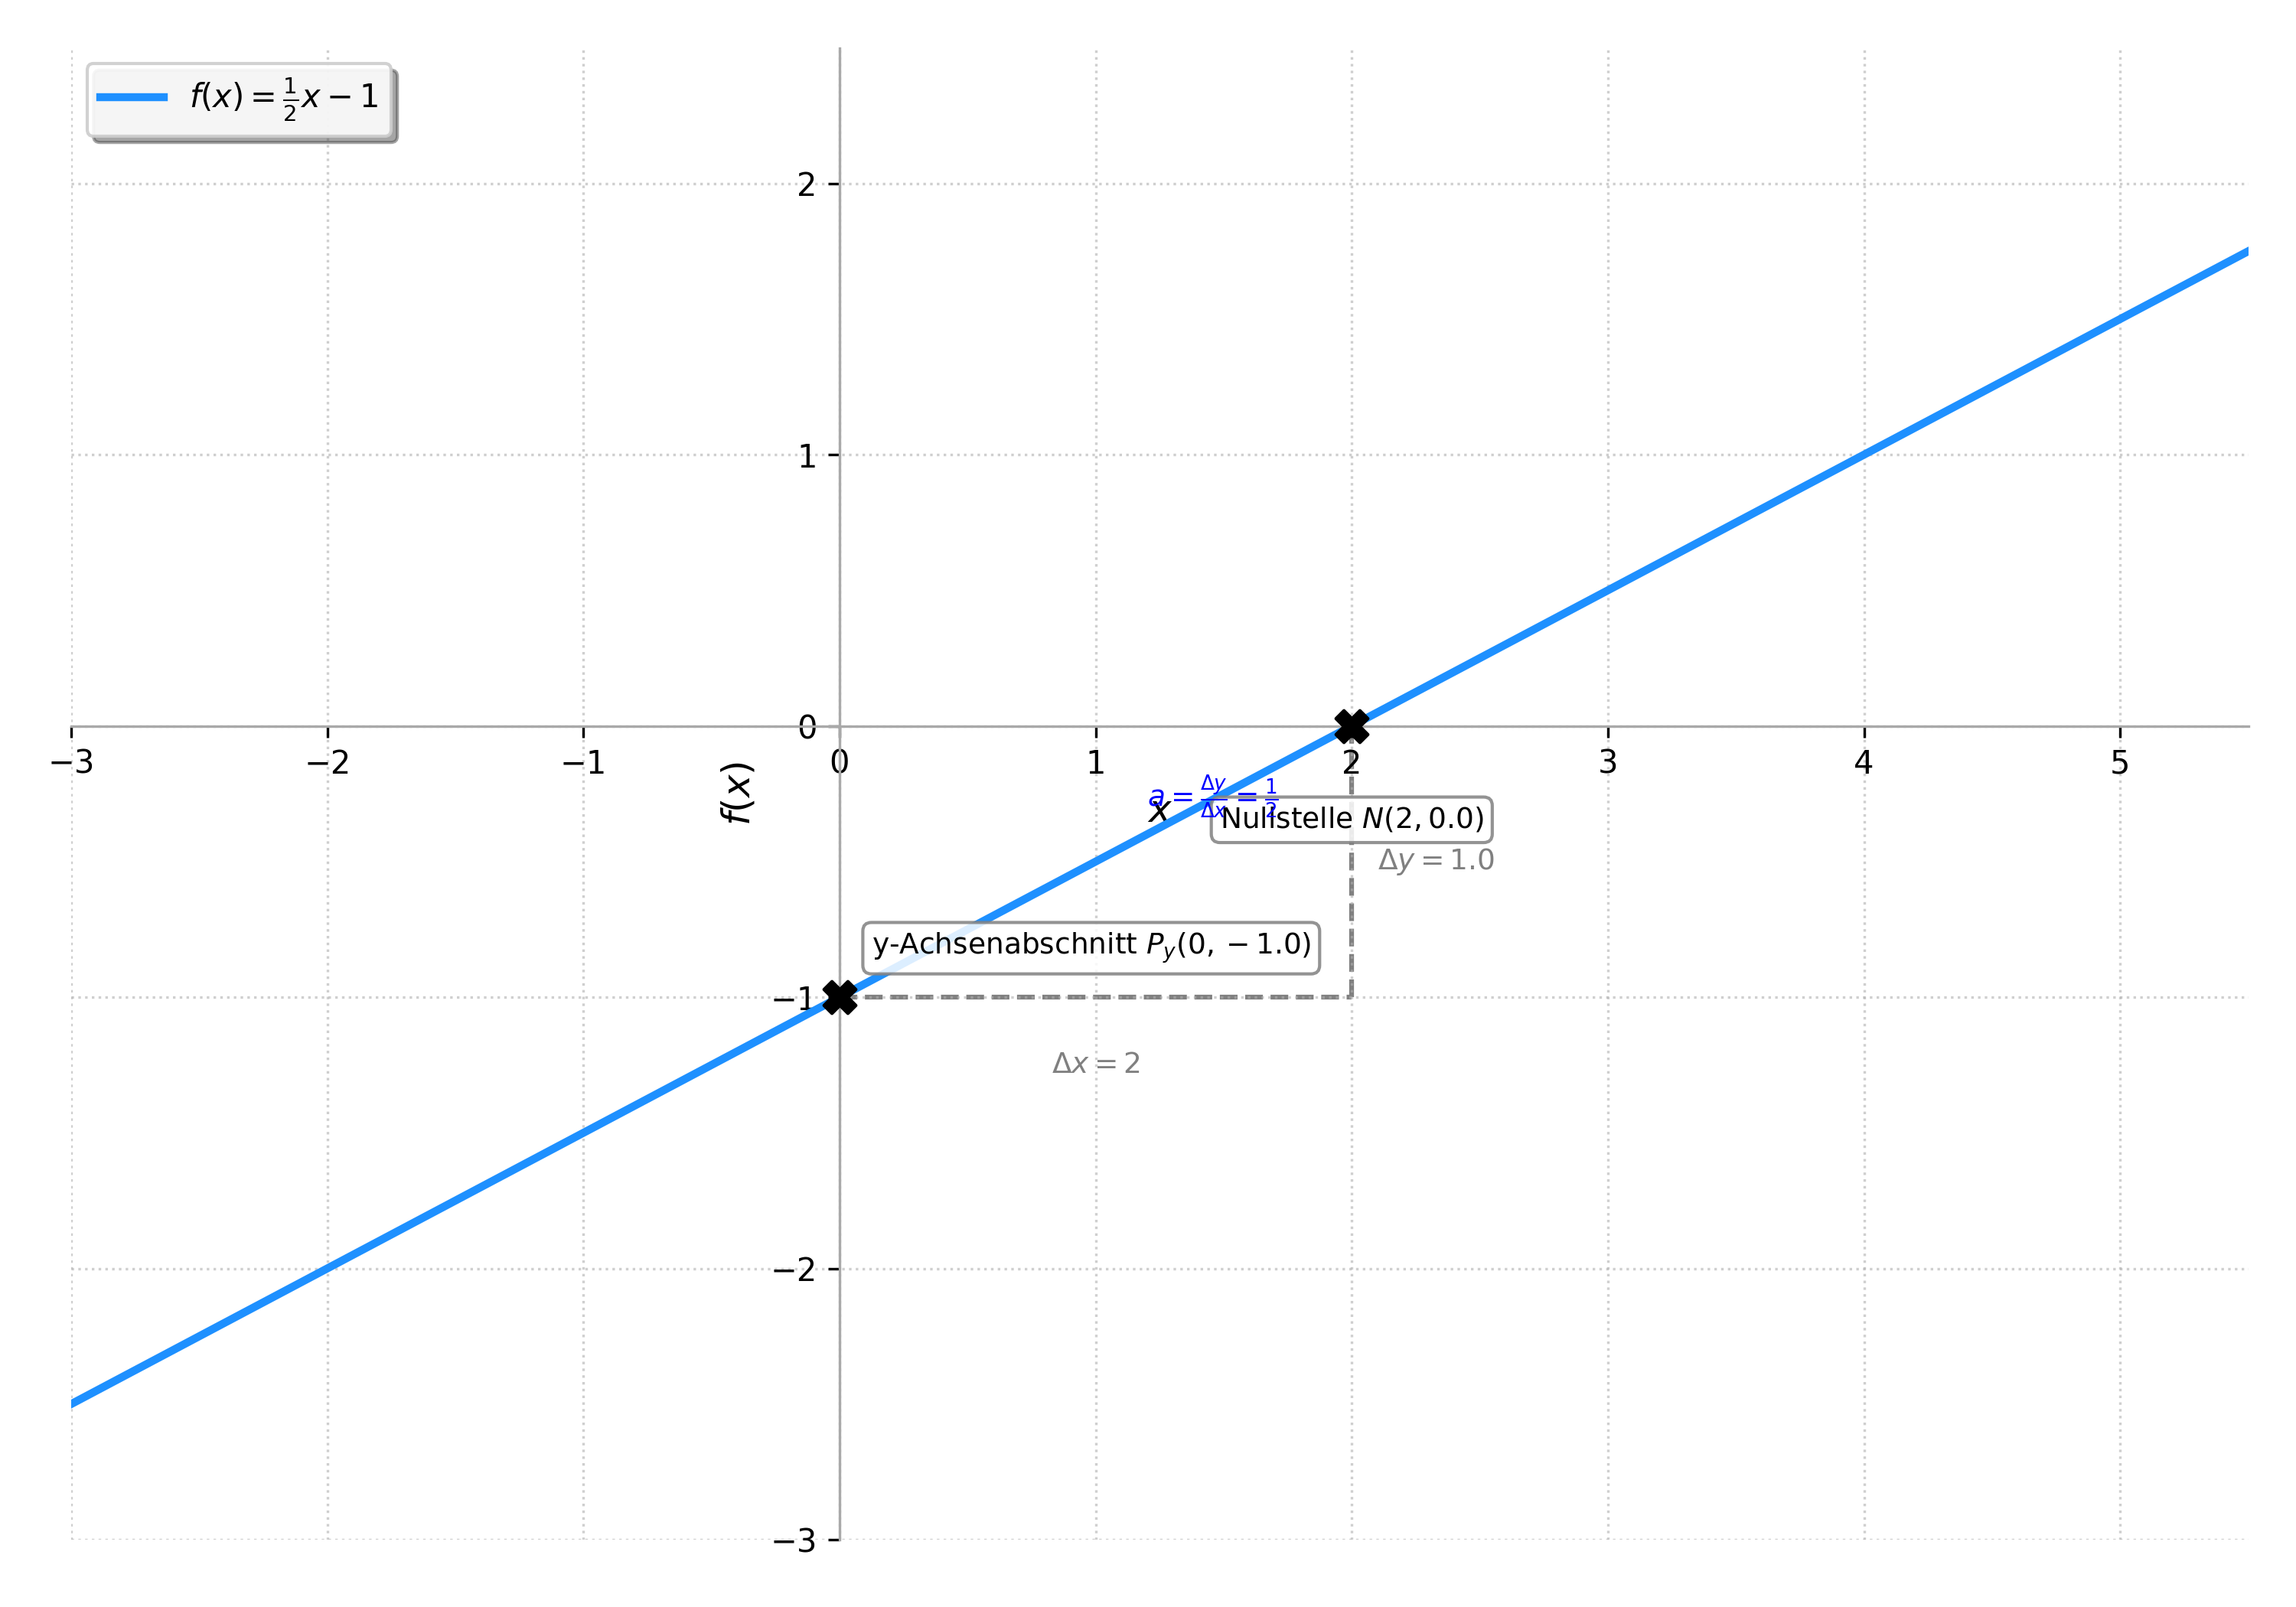
\includegraphics[width=0.8\textwidth]{grafiken/funktion_checkliste_graph.png}
    % --- Beschreibung der Grafik ---
    % Die Grafik zeigt ein kartesisches Koordinatensystem.
    % Die x-Achse und y-Achse sind beschriftet und sinnvoll skaliert (z.B. von -3 bis 5 für x und -3 bis 2 für y).
    % Eingezeichnet ist der Graph der Funktion f(x) = (1/2)x - 1. Es ist eine Gerade.
    % Die Nullstelle (Schnittpunkt mit der x-Achse) bei (2|0) ist deutlich markiert.
    % Der y-Achsenabschnitt (Schnittpunkt mit der y-Achse) bei (0|-1) ist deutlich markiert.
    % Die Gerade steigt an, was der positiven Steigung a=1/2 entspricht.
    % Ein Steigungsdreieck könnte optional eingezeichnet sein (z.B. 2 Einheiten nach rechts, 1 Einheit nach oben).
    \captionof{figure}{Graph der Funktion $f(x) = \frac{1}{2}x - 1$ mit markierter Nullstelle und y-Achsenabschnitt.}
    \label{fig:checkliste_graph}
    \end{center}
    Der Graph ist eine Gerade, die die y-Achse bei $y=-1$ schneidet und die x-Achse bei $x=2$. Da die Steigung $a=\frac{1}{2}$ positiv ist, steigt die Gerade an.

    \item \textbf{Funktionswerte positiv/negativ:}
    Die Nullstelle der Funktion ist $x_0=2$.
    \begin{itemize}
        \item Für welche $x$-Werte sind die Funktionswerte $f(x)$ \textbf{positiv}? \\
        Da die Funktion eine positive Steigung hat ($a=\frac{1}{2} > 0$) und bei $x_0=2$ die x-Achse schneidet (also $f(2)=0$), sind die Funktionswerte für alle $x$-Werte rechts von der Nullstelle positiv.
        Der Graph verläuft oberhalb der x-Achse für $x > 2$. Bereich: $(2, \infty)$.
        \item Für welche $x$-Werte sind die Funktionswerte $f(x)$ \textbf{negativ}? \\
        Entsprechend sind die Funktionswerte für alle $x$-Werte links von der Nullstelle negativ.
        Der Graph verläuft unterhalb der x-Achse für $x < 2$. Bereich: $(-\infty, 2)$.
    \end{itemize}

    \item \textbf{Rolle der Steigung:}
    Die Steigung $a = \frac{1}{2}$ ist positiv. Das bedeutet, dass die Funktion streng monoton steigt: Wenn $x$ größer wird, wird auch $f(x)$ größer.
    Sobald man die Nullstelle $x_0$ kennt (dort ist $f(x_0)=0$), hilft die positive Steigung wie folgt:
    \begin{itemize}
        \item Für $x$-Werte, die größer als die Nullstelle sind ($x > x_0$), müssen die Funktionswerte größer als $f(x_0)=0$ sein, also $f(x) > 0$ (positiv). Man bewegt sich auf der Geraden von der Nullstelle aus nach rechts und oben.
        \item Für $x$-Werte, die kleiner als die Nullstelle sind ($x < x_0$), müssen die Funktionswerte kleiner als $f(x_0)=0$ sein, also $f(x) < 0$ (negativ). Man bewegt sich auf der Geraden von der Nullstelle aus nach links und unten.
    \end{itemize}
    Wäre die Steigung negativ, wäre das Verhalten genau umgekehrt.

    \item \textbf{Rolle des y-Achsenabschnitts:}
    Der y-Achsenabschnitt ist $b=-1$. Das bedeutet, $f(0)=-1$. Dieser Wert gibt uns direkt einen Punkt auf dem Graphen an, nämlich $(0|-1)$.
    Da $f(0)=-1$ negativ ist, wissen wir, dass der Graph der Funktion an der Stelle $x=0$ (also auf der y-Achse) unterhalb der x-Achse verläuft.
    Für $x$-Werte 'nahe Null' (z.B. im Intervall $(-1,1)$), die links von der Nullstelle $x_0=2$ liegen, können wir erwarten, dass die Funktionswerte negativ sind, da die Funktion stetig ist und von $f(0)=-1$ aus mit positiver Steigung zur Nullstelle $f(2)=0$ ansteigt. Der y-Achsenabschnitt ist also ein konkreter Funktionswert, der hilft, das Vorzeichen von $f(x)$ in der Umgebung von $x=0$ zu bestimmen und die Lage des Graphen zu verorten.

    \item \textbf{Wertebereich:}
    Der Wertebereich einer nicht-konstanten linearen Funktion wie $f(x) = \frac{1}{2}x - 1$ ist die Menge aller reellen Zahlen, geschrieben als $\mathbb{R}$.
    Am Graphen kann man dies erkennen, da die Gerade sich unendlich weit nach oben und nach unten fortsetzt.
    \begin{itemize}
        \item Wenn man auf der x-Achse sehr weit nach rechts geht (große positive $x$-Werte), werden die $y$-Werte ($f(x)$) beliebig groß positiv (z.B. $f(1000) = \frac{1}{2}(1000)-1 = 499$).
        \item Wenn man auf der x-Achse sehr weit nach links geht (große negative $x$-Werte), werden die $y$-Werte ($f(x)$) beliebig klein negativ (z.B. $f(-1000) = \frac{1}{2}(-1000)-1 = -501$).
    \end{itemize}
    Da die Funktion stetig ist (keine Sprünge oder Lücken hat) und in beide Richtungen unbeschränkt wächst bzw. fällt, wird jeder reelle y-Wert irgendwann einmal als Funktionswert angenommen. Man kann für jeden beliebigen y-Zielwert $y_{Ziel}$ die Gleichung $y_{Ziel} = \frac{1}{2}x - 1$ nach $x$ auflösen ($x = 2(y_{Ziel}+1)$) und erhält immer einen entsprechenden $x$-Wert.
\end{enumerate}

\end{loesungsumgebung}


\begin{aufgabenumgebung}{Checkliste: Verhalten linearer Funktionen verstehen und interpretieren}
Gegeben sei die lineare Funktion $g(x) = -2x + 4$.
Führe eine Analyse dieser Funktion anhand der folgenden Punkte durch:

\begin{enumerate}[label=(\alph*)]
    \item \textbf{Nullstelle und y-Achsenabschnitt:} Berechne die Nullstelle von $g(x)$ und gib den y-Achsenabschnitt an.
    \item \textbf{Skizze:} Zeichne den Graphen der Funktion $g(x)$. Achte darauf, die Achsenschnittpunkte klar zu kennzeichnen.
    \item \textbf{Vorzeichen der Funktionswerte:}
    \begin{itemize}
        \item In welchem Intervall ist $g(x) > 0$?
        \item In welchem Intervall ist $g(x) < 0$?
    \end{itemize}
    \item \textbf{Argumentation mit Steigung und Nullstelle:} Erkläre, wie du allein aus dem Vorzeichen der Steigung $a=-2$ und der Lage der Nullstelle $x_0$ schlussfolgern kannst, ob die Funktionswerte für $x$-Werte, die größer als die Nullstelle sind ($x > x_0$), positiv oder negativ sein müssen.
    \item \textbf{Vergleich mit dem y-Achsenabschnitt:} Bestätigt der y-Achsenabschnitt deine Überlegungen zum Vorzeichen der Funktion für $x=0$? Liegt $x=0$ in dem von dir bestimmten positiven oder negativen Bereich?
    \item \textbf{Gedankenexperiment:} Stell dir eine lineare Funktion $h(x)$ vor, von der du nur weißt: Ihre Steigung ist positiv ($a > 0$) und ihre Nullstelle ist ebenfalls positiv ($x_0 > 0$).
    \begin{itemize}
        \item Mache eine grobe Skizze, wie solch eine Funktion aussehen könnte.
        \item Welches Vorzeichen muss der y-Achsenabschnitt dieser Funktion $h(x)$ haben? Begründe deine Antwort mathematisch oder anhand deiner Skizze.
    \end{itemize}
\end{enumerate}
\end{aufgabenumgebung}


\begin{loesungsumgebung}[loes:checkliste-verhalten-linearer-funktionen]{Checkliste: Verhalten lin. Funktionen verstehen und interpretieren}
Wir analysieren die lineare Funktion $g(x) = -2x + 4$.

\begin{enumerate}[label=(\alph*)]
    \item \textbf{Nullstelle und y-Achsenabschnitt:}
    \begin{itemize}
        \item \textbf{Y-Achsenabschnitt:} Der y-Achsenabschnitt $b$ ist der konstante Term in der Funktionsgleichung $g(x) = ax+b$. Für $g(x) = -2x + 4$ ist $b = 4$. Der Schnittpunkt mit der y-Achse ist also $S_y(0|4)$.
        \item \textbf{Nullstelle $x_0$:} Wir setzen $g(x_0)=0$:
        $$ -2x_0 + 4 = 0 $$
        Umformungsschritte:
        $$
        \begin{array}{r c l c l}
        \umformung{-2x_0 + 4}{0}{-}{4}
        \umformung{-2x_0}{-4}{\div}{(-2)}
        \umformungend{x_0}{2}
        \end{array}
        $$
        Die Nullstelle ist $x_0 = 2$. Der Schnittpunkt mit der x-Achse ist $S_x(2|0)$.
    \end{itemize}

    \item \textbf{Skizze:}
    \begin{center}
    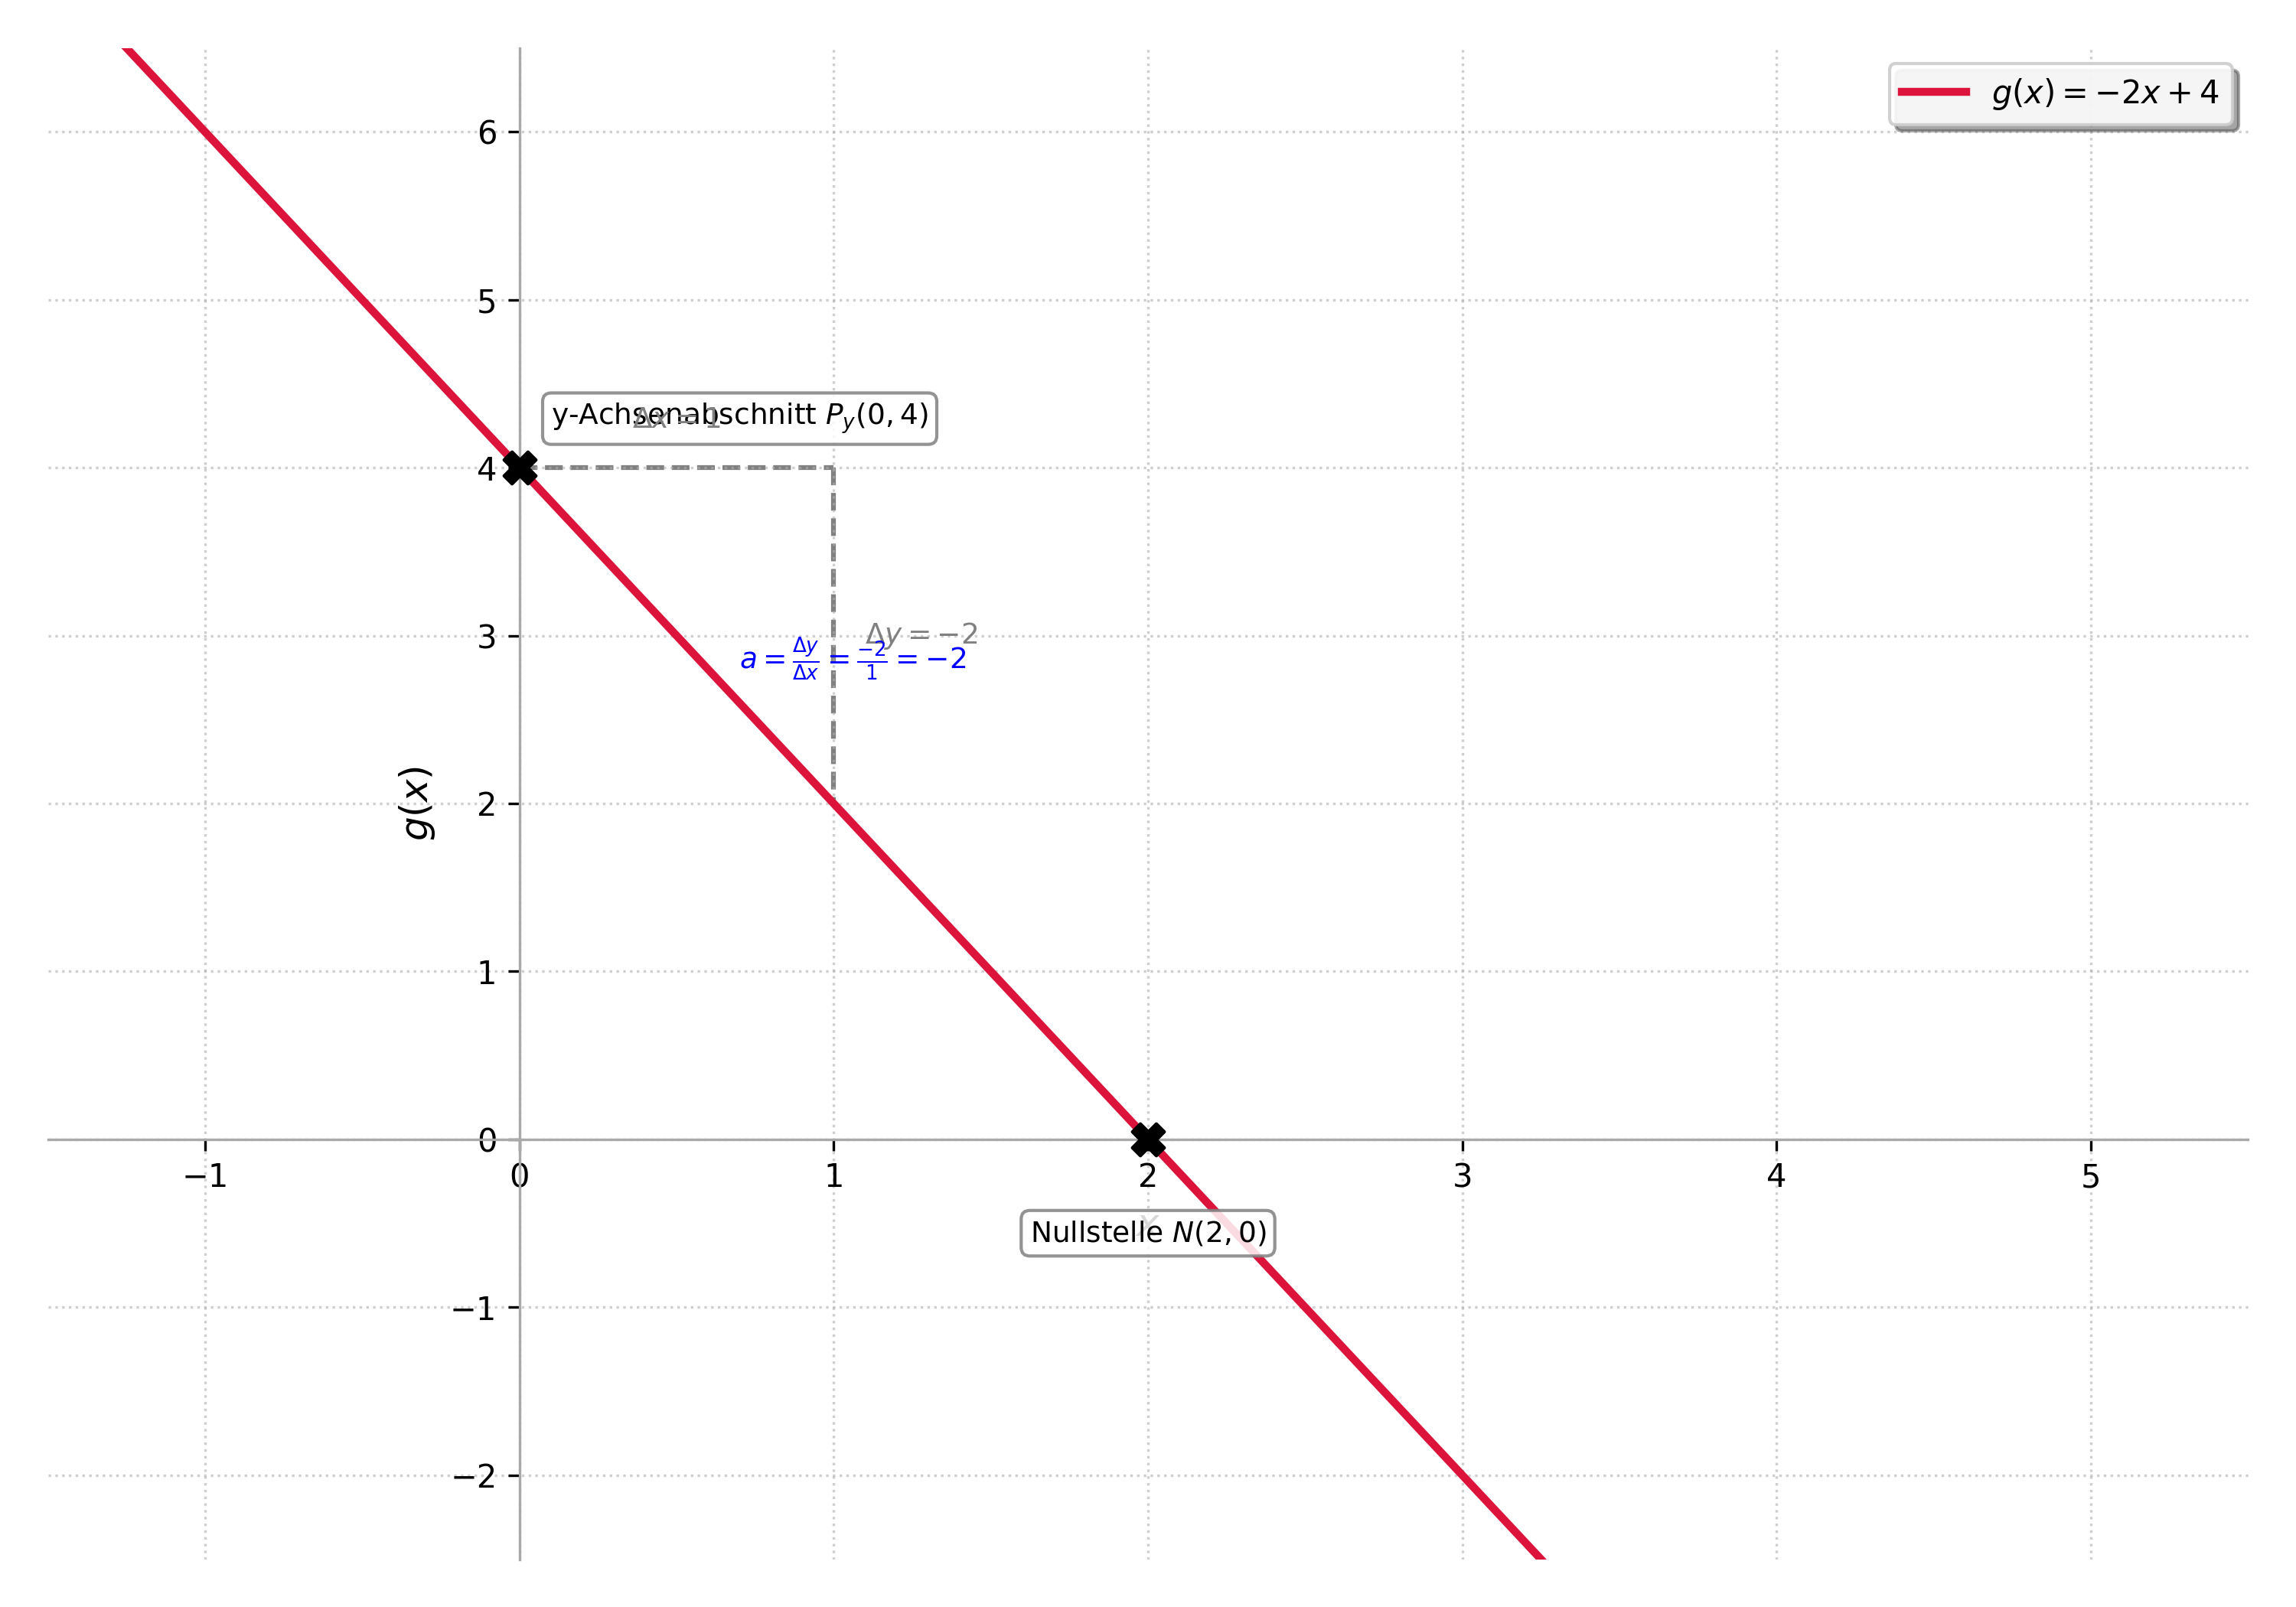
\includegraphics[width=0.8\textwidth]{grafiken/funktion_g_checkliste_graph.png}
    % --- Beschreibung der Grafik für g(x) ---
    % Die Grafik zeigt ein kartesisches Koordinatensystem.
    % Die x-Achse und y-Achse sind beschriftet und sinnvoll skaliert (z.B. von -1 bis 5 für x und -2 bis 6 für y).
    % Eingezeichnet ist der Graph der Funktion g(x) = -2x + 4. Es ist eine Gerade.
    % Die Nullstelle (Schnittpunkt mit der x-Achse) bei (2|0) ist deutlich markiert.
    % Der y-Achsenabschnitt (Schnittpunkt mit der y-Achse) bei (0|4) ist deutlich markiert.
    % Die Gerade fällt, was der negativen Steigung a=-2 entspricht.
    % Ein Steigungsdreieck könnte optional eingezeichnet sein (z.B. 1 Einheit nach rechts, 2 Einheiten nach unten).
    \captionof{figure}{Graph der Funktion $g(x) = -2x + 4$ mit markierten Achsenschnittpunkten.}
    \label{fig:g_checkliste_graph}
    \end{center}
    Der Graph ist eine Gerade, die die y-Achse bei $y=4$ und die x-Achse bei $x=2$ schneidet. Da die Steigung $a=-2$ negativ ist, fällt die Gerade.

    \item \textbf{Vorzeichen der Funktionswerte:}
    Die Nullstelle der Funktion ist $x_0=2$. Die Steigung ist $a=-2$ (negativ).
    \begin{itemize}
        \item \textbf{In welchem Intervall ist $g(x) > 0$?} \\
        Da die Funktion eine negative Steigung hat und bei $x_0=2$ die x-Achse schneidet (also $g(2)=0$), sind die Funktionswerte für alle $x$-Werte links von der Nullstelle positiv (die Gerade kommt von 'oben links').
        Der Graph verläuft oberhalb der x-Achse für $x < 2$. Intervall: $(-\infty, 2)$.
        \item \textbf{In welchem Intervall ist $g(x) < 0$?} \\
        Entsprechend sind die Funktionswerte für alle $x$-Werte rechts von der Nullstelle negativ.
        Der Graph verläuft unterhalb der x-Achse für $x > 2$. Intervall: $(2, \infty)$.
    \end{itemize}

    \item \textbf{Argumentation mit Steigung und Nullstelle:}
    Die Steigung $a=-2$ ist negativ. Das bedeutet, dass die Funktion streng monoton fällt: Wenn $x$ größer wird, wird $g(x)$ kleiner.
    Die Nullstelle ist $x_0=2$, an dieser Stelle ist $g(x_0)=0$.
    Für $x$-Werte, die größer als die Nullstelle sind ($x > x_0$), also rechts von $x_0=2$: Da die Funktion fällt, müssen die Funktionswerte $g(x)$ kleiner sein als der Wert an der Nullstelle ($g(x_0)=0$). Somit muss $g(x) < 0$ (negativ) sein für $x > x_0$.
    (Umgekehrt gilt: Für $x < x_0$ müssen die Funktionswerte größer als $g(x_0)=0$ sein, also $g(x) > 0$ (positiv).)

    \item \textbf{Vergleich mit dem y-Achsenabschnitt:}
    Der y-Achsenabschnitt ist $b=4$, das bedeutet $g(0)=4$.
    Der Funktionswert $g(0)=4$ ist positiv.
    Die Stelle $x=0$ liegt im Intervall $(-\infty, 2)$, für das wir in Teil (c) bestimmt haben, dass $g(x) > 0$ ist.
    Dies bestätigt unsere Überlegungen: Da $x=0 < x_0=2$ ist (also links von der Nullstelle liegt) und die Funktion eine negative Steigung hat (also von links oben nach rechts unten verläuft), muss der Funktionswert bei $x=0$ positiv sein.

    \item \textbf{Gedankenexperiment:}
    Wir stellen uns eine lineare Funktion $h(x)$ vor mit: Steigung $a_h > 0$ (positiv) und Nullstelle $x_{h0} > 0$ (positiv).
    \begin{itemize}
        \item \textbf{Grobe Skizze, wie solch eine Funktion aussehen könnte.}
        \begin{center}
        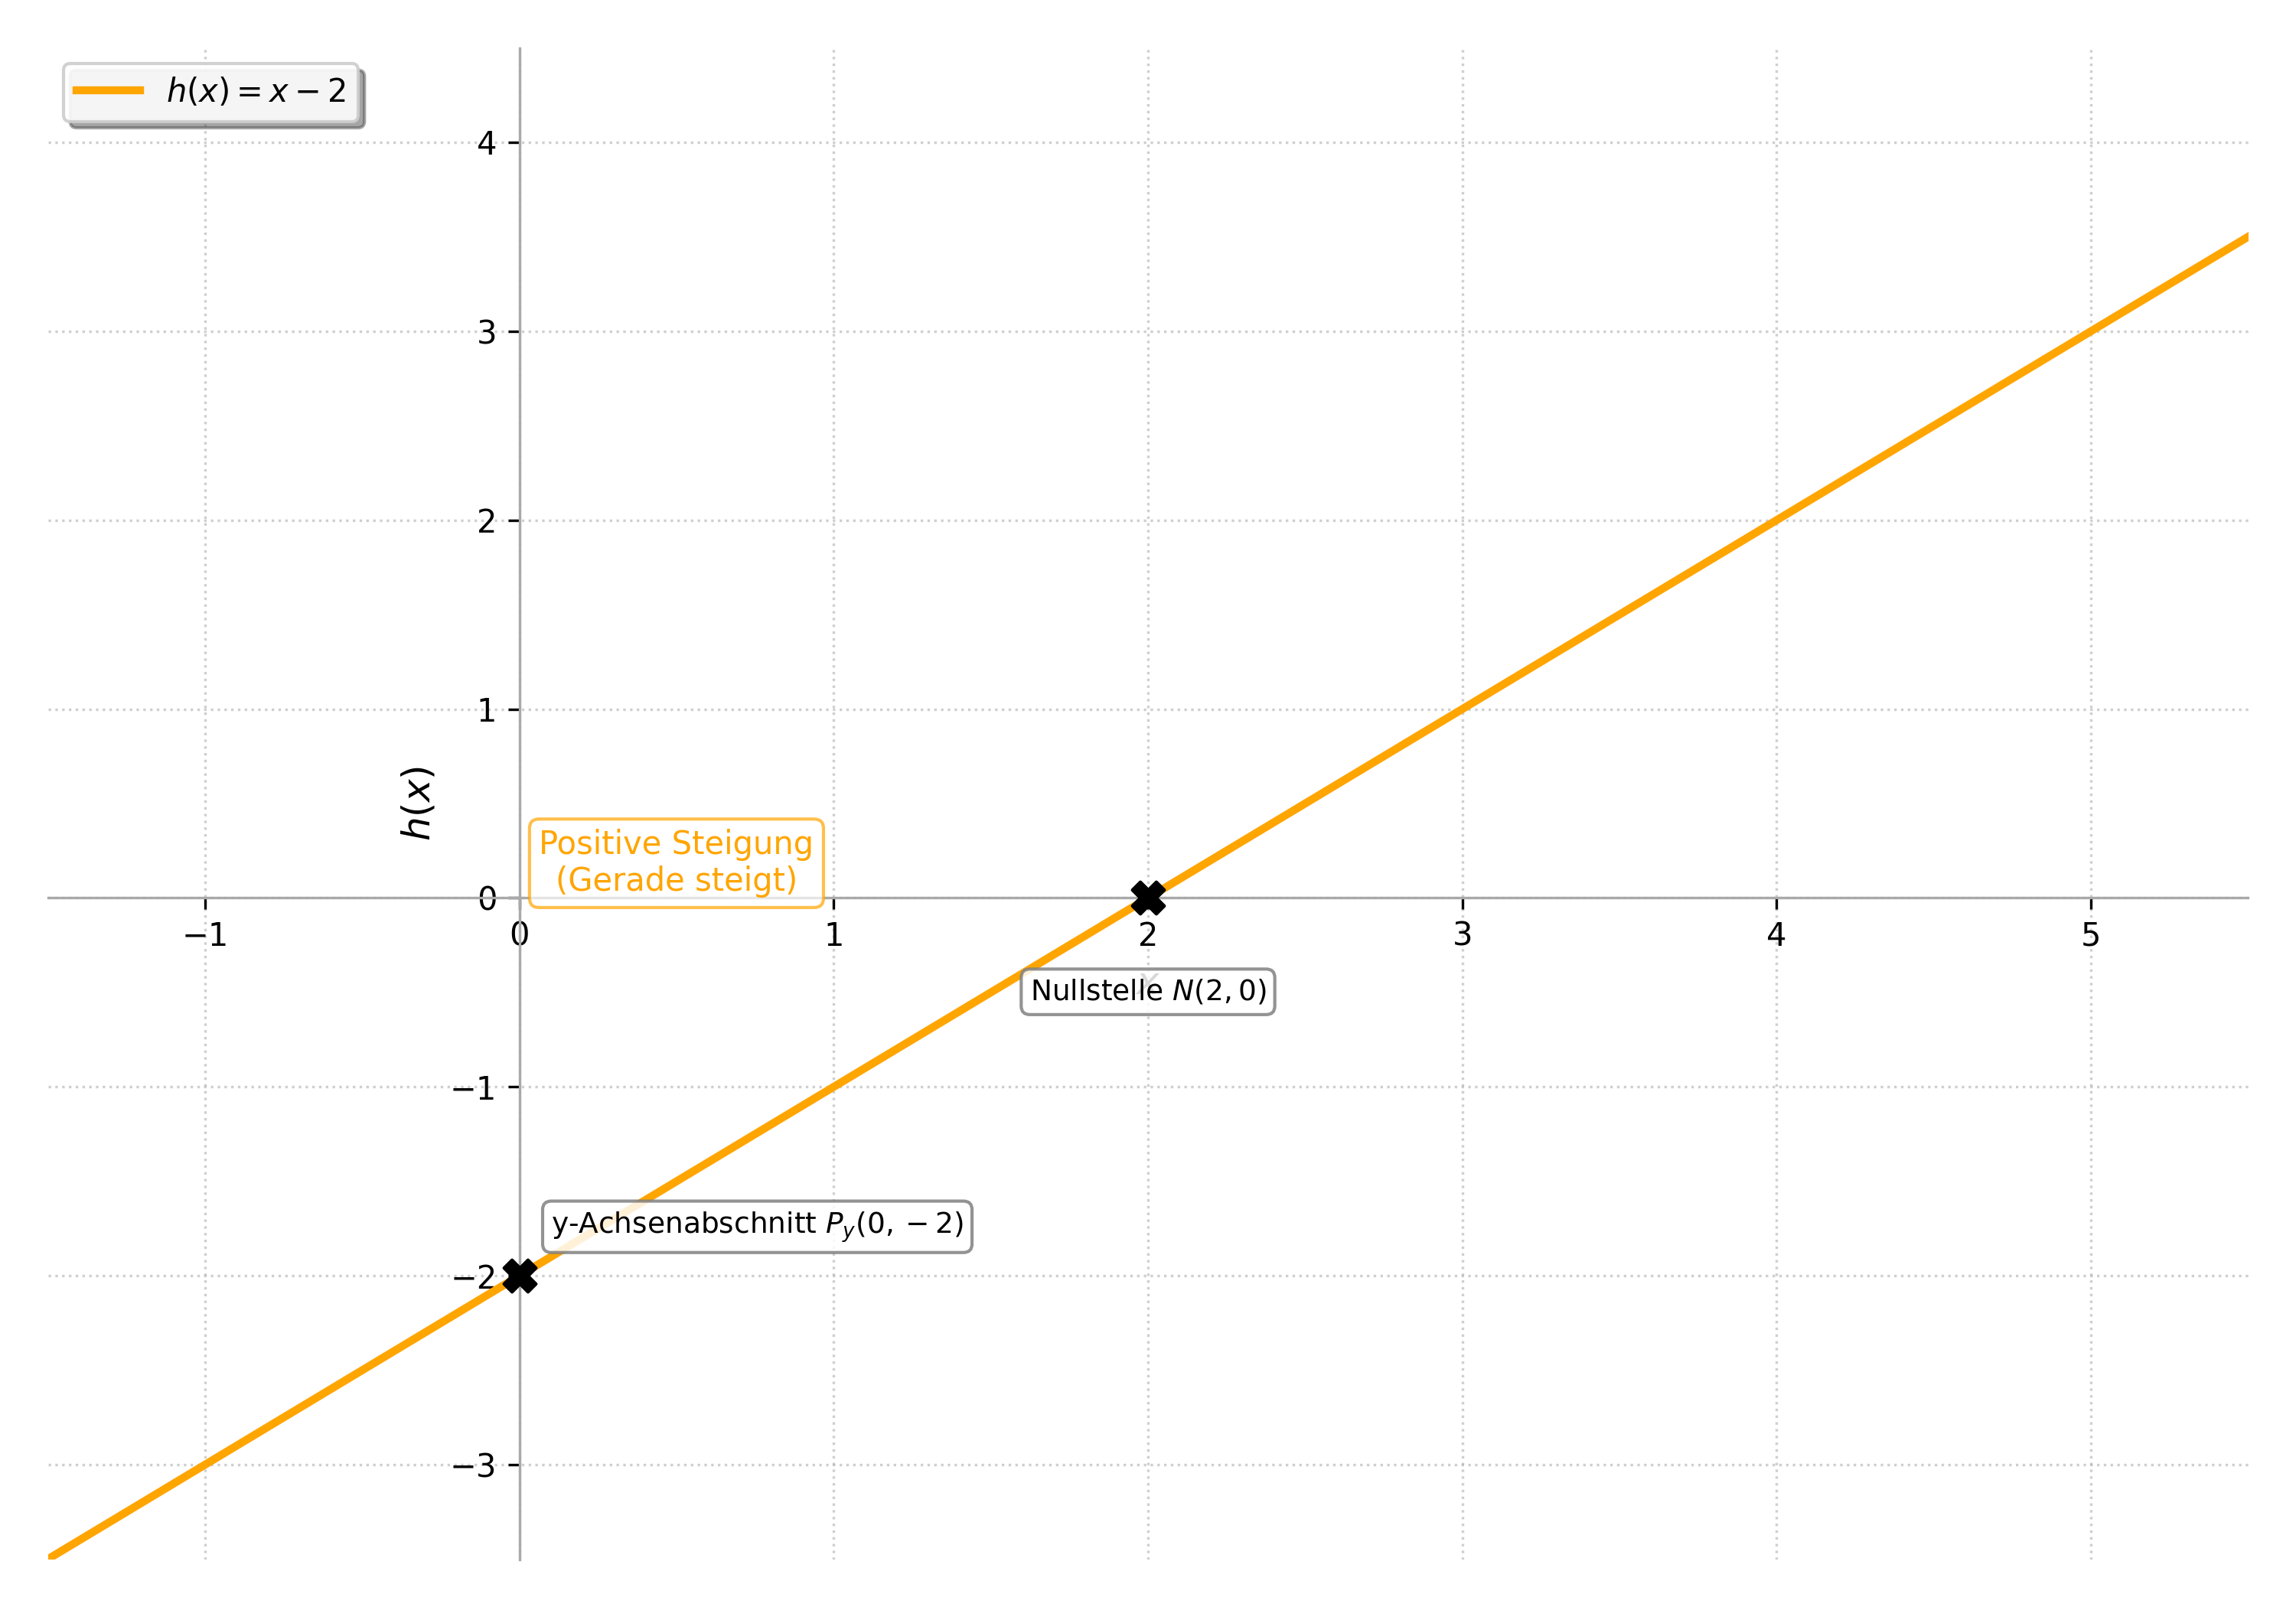
\includegraphics[width=0.8\textwidth]{grafiken/funktion_h_gedankenexperiment_graph.png}
        % --- Beschreibung der Grafik für h(x) ---
        % Die Grafik zeigt ein kartesisches Koordinatensystem.
        % Eine Gerade h(x) ist eingezeichnet, die von links unten nach rechts oben steigt (positive Steigung).
        % Diese Gerade schneidet die x-Achse im positiven Bereich (rechts vom Ursprung, da x_h0 > 0).
        % Folglich muss die Gerade die y-Achse unterhalb des Ursprungs schneiden.
        \captionof{figure}{Skizze einer linearen Funktion $h(x)$ mit positiver Steigung und positiver Nullstelle.}
        \label{fig:h_gedankenexperiment_graph}
        \end{center}

        \item \textbf{Welches Vorzeichen muss der y-Achsenabschnitt dieser Funktion $h(x)$ haben? Begründe.} \\
        Der y-Achsenabschnitt $b_h$ dieser Funktion $h(x)$ muss \textbf{negativ} sein.

        \textbf{Begründung anhand der Skizze:}
        Wenn eine Gerade eine positive Steigung hat (also von links unten nach rechts oben verläuft) und ihre Nullstelle im positiven $x$-Bereich liegt (d.h., sie schneidet die x-Achse rechts vom Ursprung), dann muss sie die y-Achse ($x=0$) unterhalb der x-Achse geschnitten haben, um diesen positiven $x$-Achsenabschnitt zu erreichen. Ein Schnittpunkt mit der y-Achse unterhalb der x-Achse bedeutet einen negativen y-Achsenabschnitt.

        \textbf{Mathematische Begründung:}
        Die allgemeine Form der linearen Funktion ist $h(x) = a_h x + b_h$.
        An der Nullstelle $x_{h0}$ gilt $h(x_{h0}) = 0$:
        $$ a_h x_{h0} + b_h = 0 $$
        Wir lösen nach dem y-Achsenabschnitt $b_h$ auf:
        $$ b_h = -a_h x_{h0} $$
        Wir wissen:
        \begin{itemize}
            \item Die Steigung $a_h$ ist positiv ($a_h > 0$).
            \item Die Nullstelle $x_{h0}$ ist positiv ($x_{h0} > 0$).
        \end{itemize}
        Das Produkt zweier positiver Zahlen $a_h \cdot x_{h0}$ ist ebenfalls positiv.
        Da $b_h = -(a_h x_{h0})$ ist, und $a_h x_{h0}$ positiv ist, muss $b_h$ negativ sein (z.B. wenn $a_h x_{h0} = 5$, dann ist $b_h = -5$).
    \end{itemize}
\end{enumerate}

\end{loesungsumgebung}